\section{Iteración 0}
\subsection{Exploración}
En éste apartado se definirá el alcance del proyecto, los recursos u herramientas a usar, y las personas involucradas en su desarrollo, así como las pruebas de contexto realizadas en las tecnologías que usaremos.


\subsubsection{Pruebas de contexto}
Con el fin de conocer las capacidades de las plataforma ARCore y Vuforia (excluyendo ARKit debido a que su desarrollo en enfocado a sistemas iOS, ARToolkit porque no se centra en dispositivos móviles y a Wikitude por su reducido número de dispositivos compatibles), se realizaron pruebas de contexto definiendo las siguientes especificaciones:
\begin{itemize}
	\item Nombre del dispositivo en el que se realizó
	\item Fecha de prueba
	\item Versión de la tecnologia SDK
	\item Versión de Android
\end{itemize}
Por otro lado cada prueba se realizó tomando en cuenta las siguientes características:
\begin{itemize}
	\item \textbf{Posición Cardinal}.- Define si un objeto virtual puede visualizarse desde los cuatro puntos cardinales (norte, sur, este, oeste) y desde la parte superior del mismo, cuando la cámara gira alrededor del objeto mientras lo enfoca.
	\item \textbf{Tamaño relativo}.- Define si un objeto cambia su tamaño en el entorno virtual dependiendo de la distancia a la que se acerque o se aleje la cámara. Cuando la cámara se acerca, el objeto deberá aumentar su tamaño, y viceversa, como si se tratase de un objeto real.
	\item \textbf{Luminosidad}.- Define el grado de oscuridad de un objeto a determinada luz, es decir, cuando la luz en el ambiente real es alta, el objeto se verá iluminado, en caso contrario cuando haya escasa luz, el objeto se oscurecerá.
	\item \textbf{Superficie}.- Describe en qué superficies el objeto virtual es puesto, si fue posible su superposición en este material y qué comportamiento tiene en cada una de estas.
	\item \textbf{Memoria de objetos}.- Define si los objetos virtuales se conservan en la memoria cuando la cámara pierde su enfoque en ellos y los vuelve a enfocar. También describe si los objetos conservaron su posición tras el re-enfoque.
	\item \textbf{Capacidad máxima de objetos}.- Define el número de objetos virtuales que pueden ser mostrados en escena sin que el rendimiento de la aplicación caiga considerablemente.
	\item \textbf{Distancia}.- Define la distancia a la que se encuentra la cámara de un objeto virtual sin que éste desaparezca o sin que su resolución baje considerablemente.
\end{itemize}
\noindent

\subsubsection{ARcore}
\begin{table}[H]
	\centering
	\begin{tabular}{|c|c|}
		\hline
		\multicolumn{2}{|c|}{Especificaciones de prueba}   \\ \hline
		\textbf{DISPOSITIVO}              & Moto G6 XT1925 \\ \hline
		\textbf{FECHA}                    & 2018/08/25     \\ \hline
		\textbf{VERSIÓN DE SCENEFORM SDK} & V1.4.0         \\ \hline
		\textbf{VERSIÓN DE ARCORE SDK}    & V1.4.0         \\ \hline
		\textbf{VERSIÓN DE ANDROID}       & V8.0.0 (Oreo)  \\ \hline
	\end{tabular}
	\captionsetup{justification=centering}
	\caption{Especificaciones de prueba Arcore en Moto G6}
\end{table}

\textbf{Posición cardinal} \par
El objeto virtual se pudo apreciar con claridad desde los cuatro puntos cardinales y la vista superior. El ángulo de visualización del objeto al mover la cámara cambiaba a la perfección, dando una buena percepción de realismo.

%%IMAGENES DE PUNTOS CARDINALES
\begin{figure}[!htbp]
	\begin{minipage}{0.48\textwidth}
	\centering
		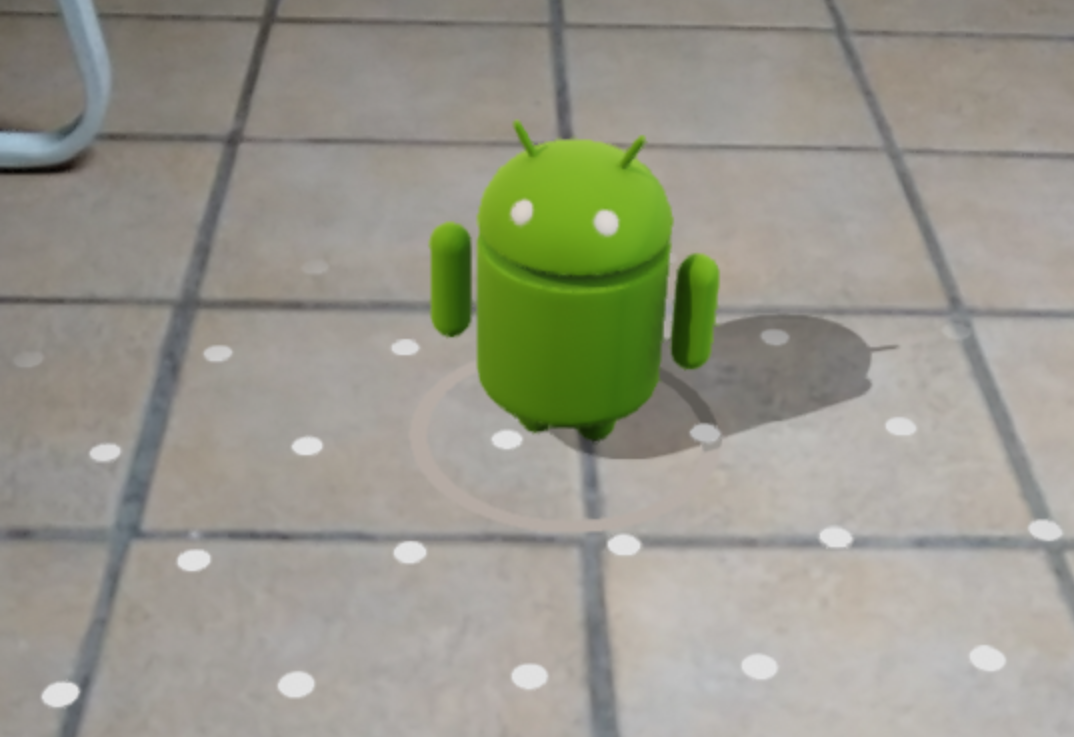
\includegraphics[width=8cm]{desarrollo/secciones/pruebas/motog6/img/NORTE.png}
		\caption{Posición Norte}
		\label{fig:motog6norte}
	\end{minipage}\hfill
	\begin{minipage}{0.48\textwidth}
	\centering
	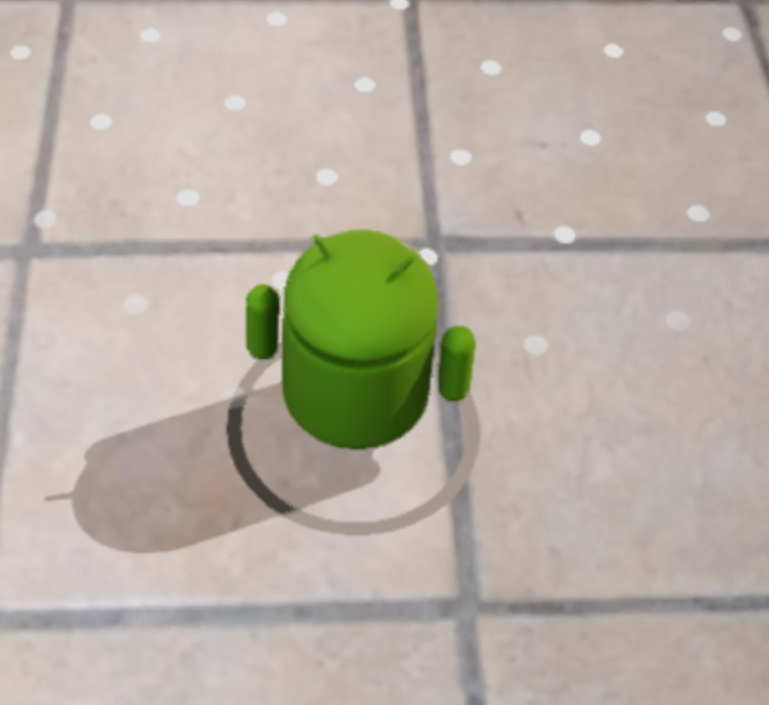
\includegraphics[width=8cm]{desarrollo/secciones/pruebas/motog6/img/SUR.png}
	\caption{Posición Sur}
	\label{fig:motog6sur}
	\end{minipage}\hfill
\end{figure}

\begin{figure}[!htbp]
	\begin{minipage}{0.48\textwidth}
		\centering
		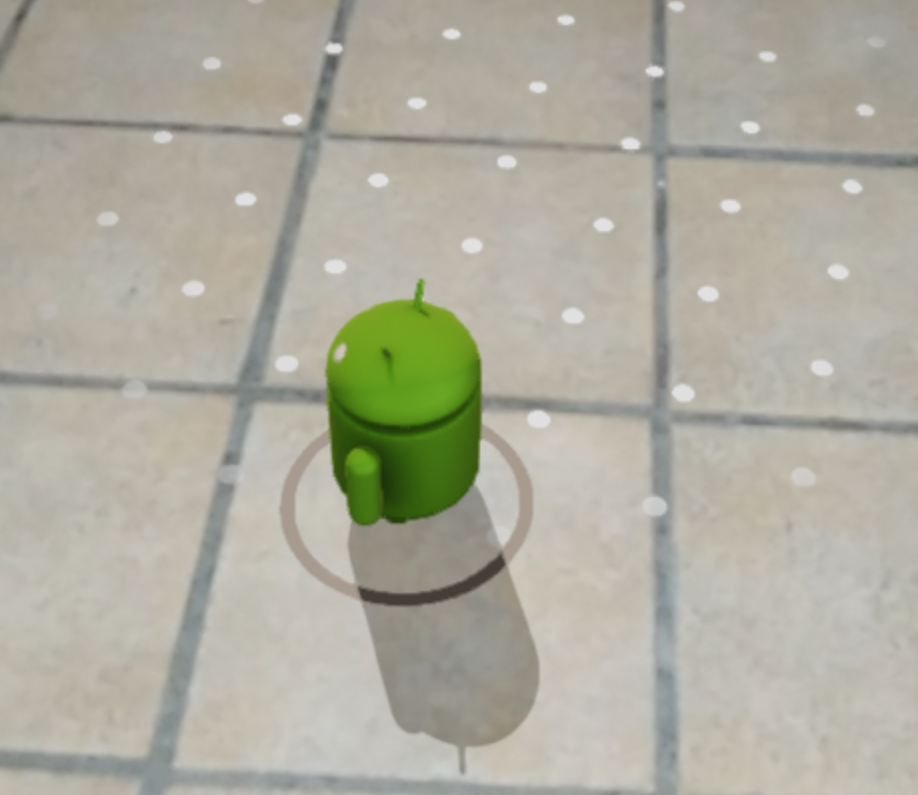
\includegraphics[width=8cm]{desarrollo/secciones/pruebas/motog6/img/ESTE.png}
		\caption{Posición Este}
		\label{fig:motog6norte}
	\end{minipage}\hfill
	\begin{minipage}{0.48\textwidth}
		\centering
		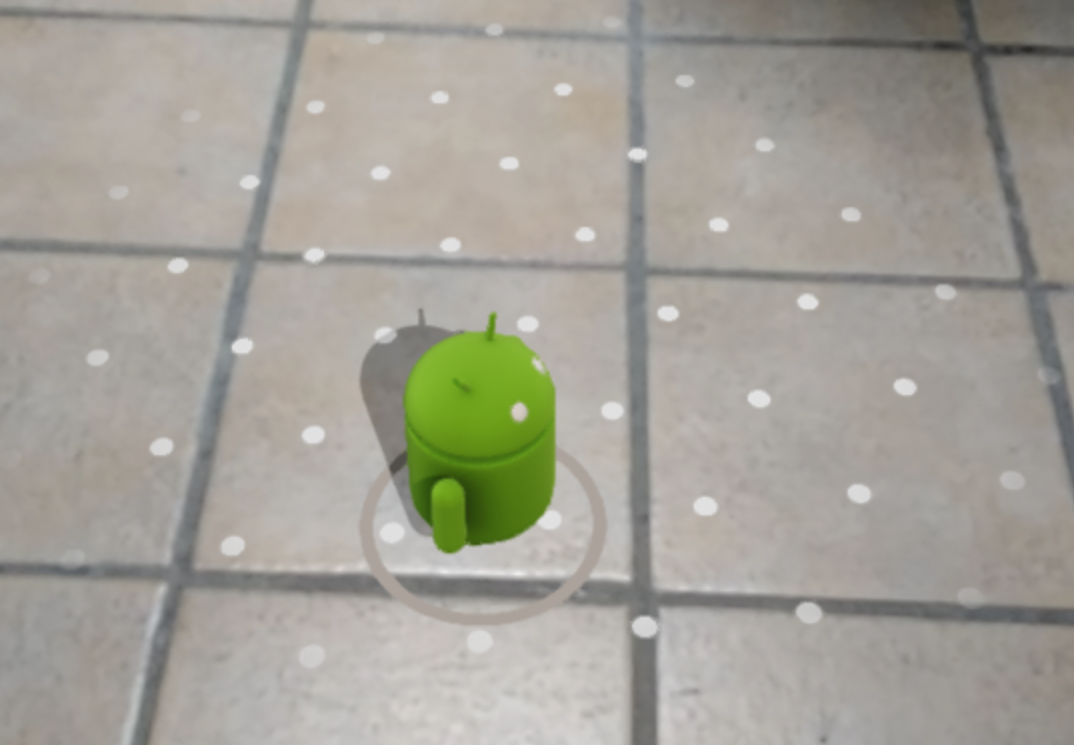
\includegraphics[width=8cm]{desarrollo/secciones/pruebas/motog6/img/OESTE.png}
		\caption{Posición Oeste}
		\label{fig:motog6oeste}
	\end{minipage}\hfill
\end{figure}

\textbf{Tamaño relativo} \par
Al acercar o alejar la cámara el objeto virtual variaba su tamaño de forma adecuada, como si el objeto realmente estuviera en la posición donde fue superpuesto.


\begin{figure}[!htbp]
	\begin{minipage}{0.48\textwidth}
		\centering
		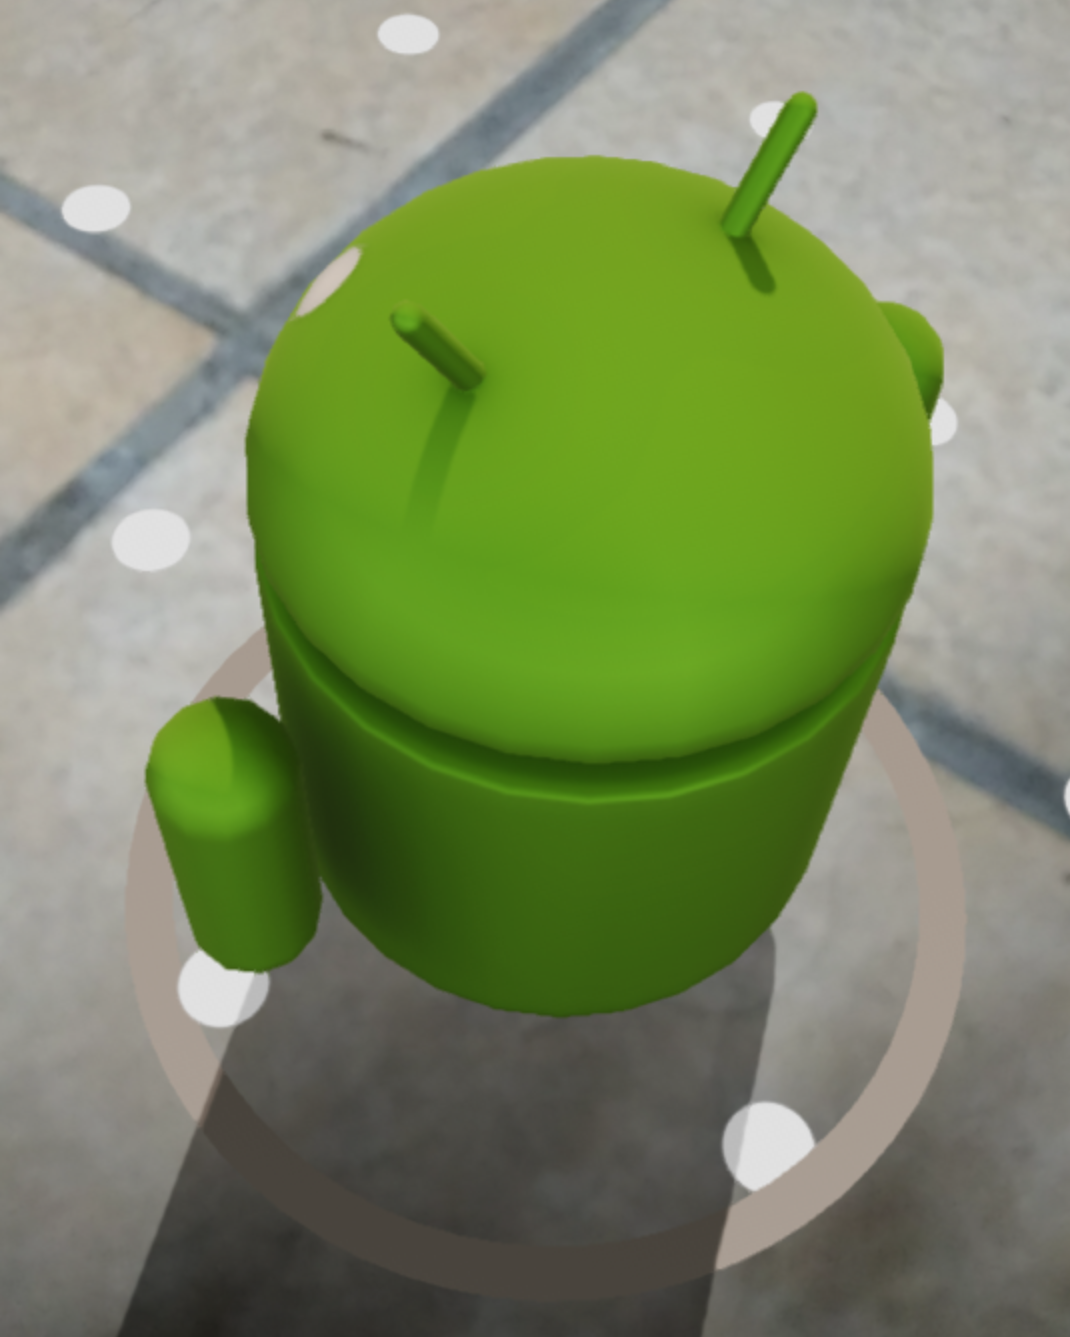
\includegraphics[width=8cm]{desarrollo/secciones/pruebas/motog6/img/CERCA.png}
		\caption{Objeto visto de cerca}
		\label{fig:motog6cerca}
	\end{minipage}\hfill
	\begin{minipage}{0.48\textwidth}
		\centering
		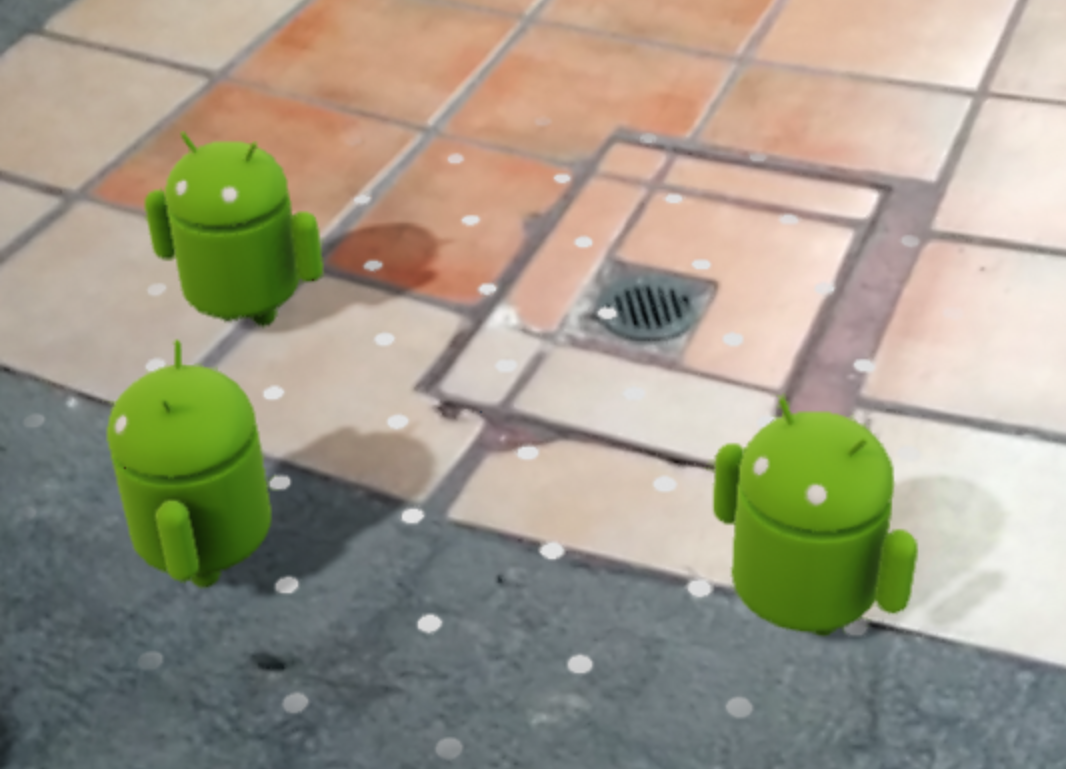
\includegraphics[width=8cm]{desarrollo/secciones/pruebas/motog6/img/LUZALTA.png}
		\caption{Luz alta}
		\label{fig:motog6lalta}
	\end{minipage}\hfill
\end{figure}

\textbf{Luminosidad} \par
Al poner el objeto virtual en entornos con diferente cantidad de luz, la cantidad de luz en el objeto virtual también variaba. En un entorno con ausencia casi total de luz el objeto apenas era perceptible, mientras que en un entorno con bastante luz, el objeto se veía altamente iluminado.

\begin{figure}[!htbp]
	\begin{minipage}{0.48\textwidth}
		\centering
		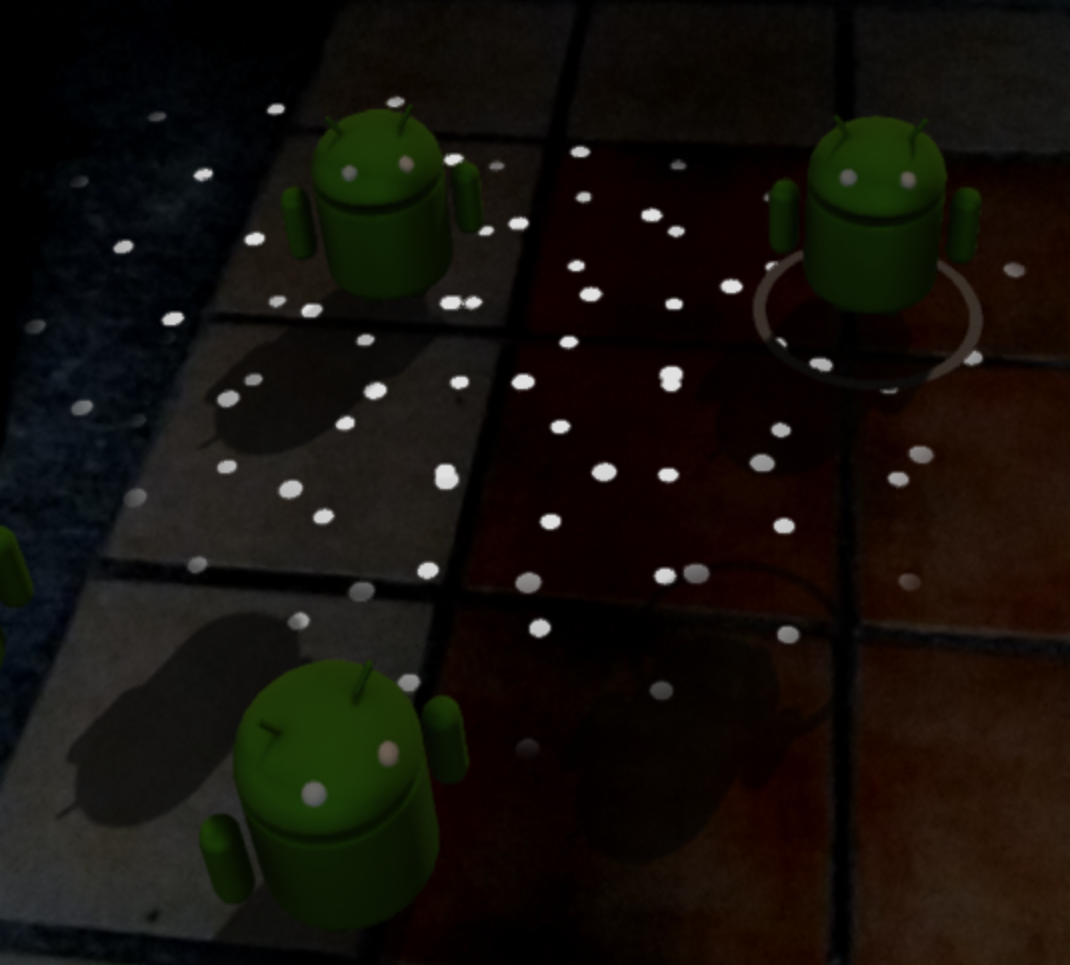
\includegraphics[width=8cm]{desarrollo/secciones/pruebas/motog6/img/LUZBAJA.png}
		\caption{Luz baja}
		\label{fig:motog6lbaja}
	\end{minipage}\hfill
	\begin{minipage}{0.48\textwidth}
		\centering
		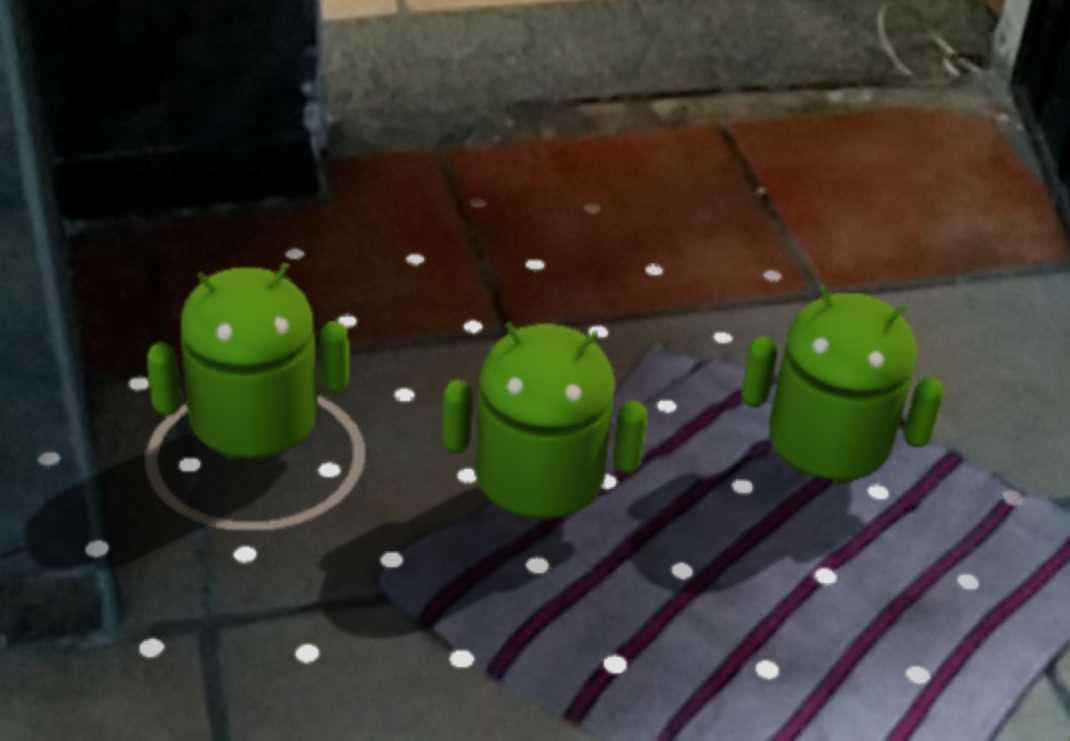
\includegraphics[width=8cm]{desarrollo/secciones/pruebas/motog6/img/LUZMEDIA.png}
		\caption{Luz media}
		\label{fig:motog6lmedia}
	\end{minipage}\hfill
\end{figure}

\textbf{Superficie} \par
Se probó posicionar el objeto virtual en cuatro superficies: concreto gris, concreto blanco, azulejo y vidrio.\par
Concreto gris.- El objeto se pudo posicionar a la perfección.\par
Concreto blanca.- El objeto no se pudo posicionar. La maya de puntos ni si quiera era detectada en ésta superficie debido a la ausencia de texturas.\par
Azulejo.- El objeto se pudo posicionar a la perfección.\par
Vidrio.- El objeto no pudo ser posicionado en ésta superficie debido a las propiedades reflejantes que posee.\par

\begin{figure}[!htbp]
	\begin{minipage}{0.48\textwidth}
		\centering
		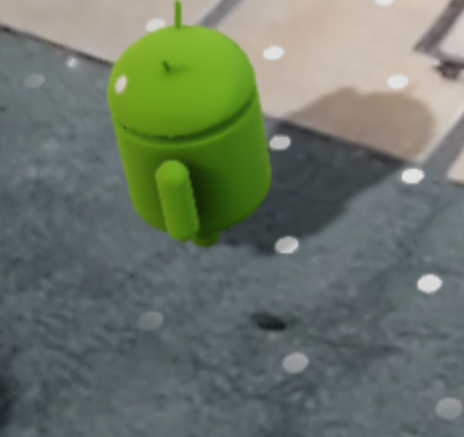
\includegraphics[width=8cm]{desarrollo/secciones/pruebas/motog6/img/CONCRETO.png}
		\caption{Objeto colocado en concreto}
		\label{fig:motog6concreto}
	\end{minipage}\hfill
	\begin{minipage}{0.48\textwidth}
		\centering
		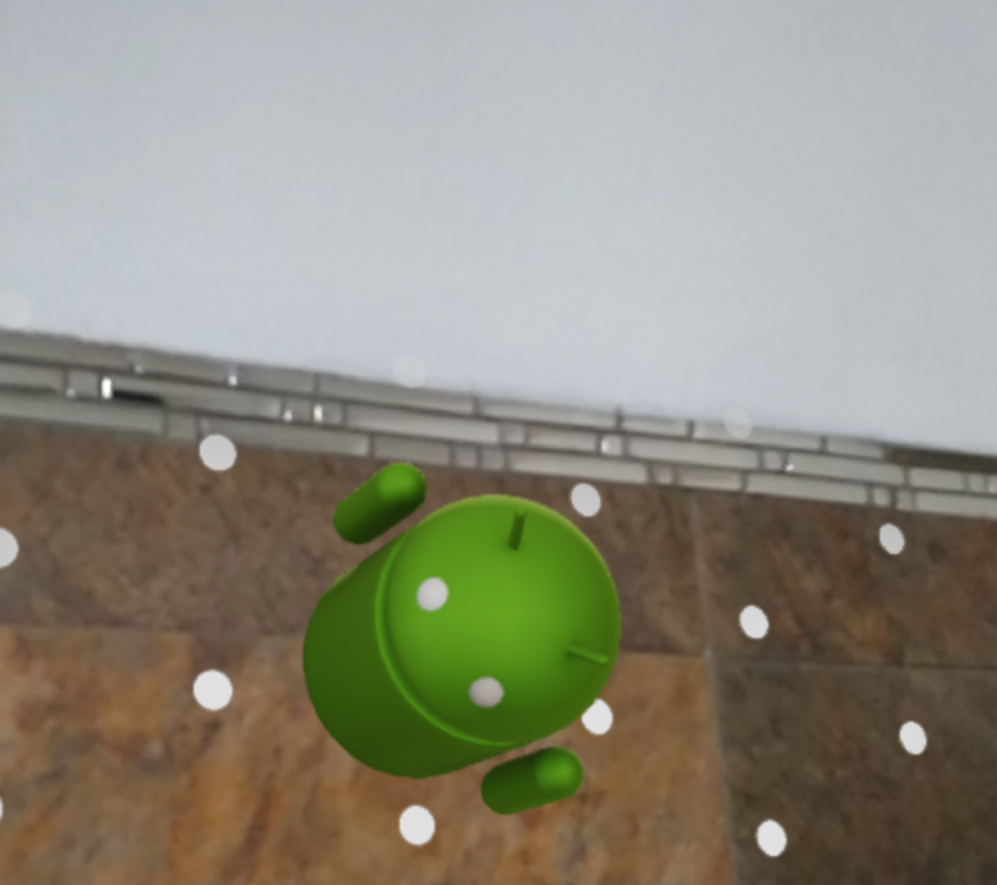
\includegraphics[width=8cm]{desarrollo/secciones/pruebas/motog6/img/SUPBLANCA.png}
		\caption{Objeto colocado en superficie blanca}
		\label{fig:motog6supblanca}
	\end{minipage}\hfill
\end{figure}

\begin{figure}[H]
	\begin{minipage}{0.48\textwidth}
		\centering
		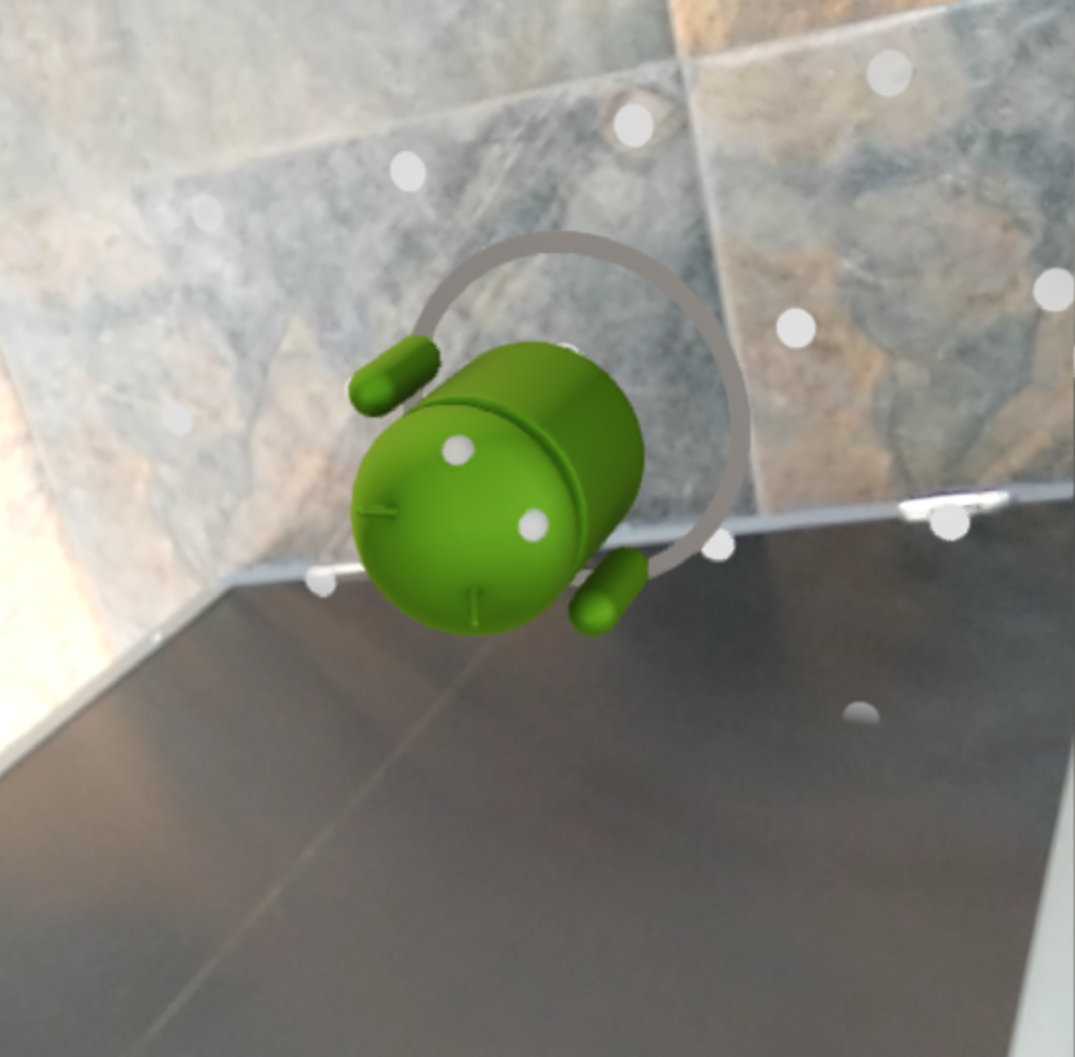
\includegraphics[width=8cm]{desarrollo/secciones/pruebas/motog6/img/SUPERFICIENEGRA.png}
		\caption{Malla de puntos no detectada en superficie negra}
		\label{fig:motog6supnegra}
	\end{minipage}\hfill
	\begin{minipage}{0.48\textwidth}
		\centering
		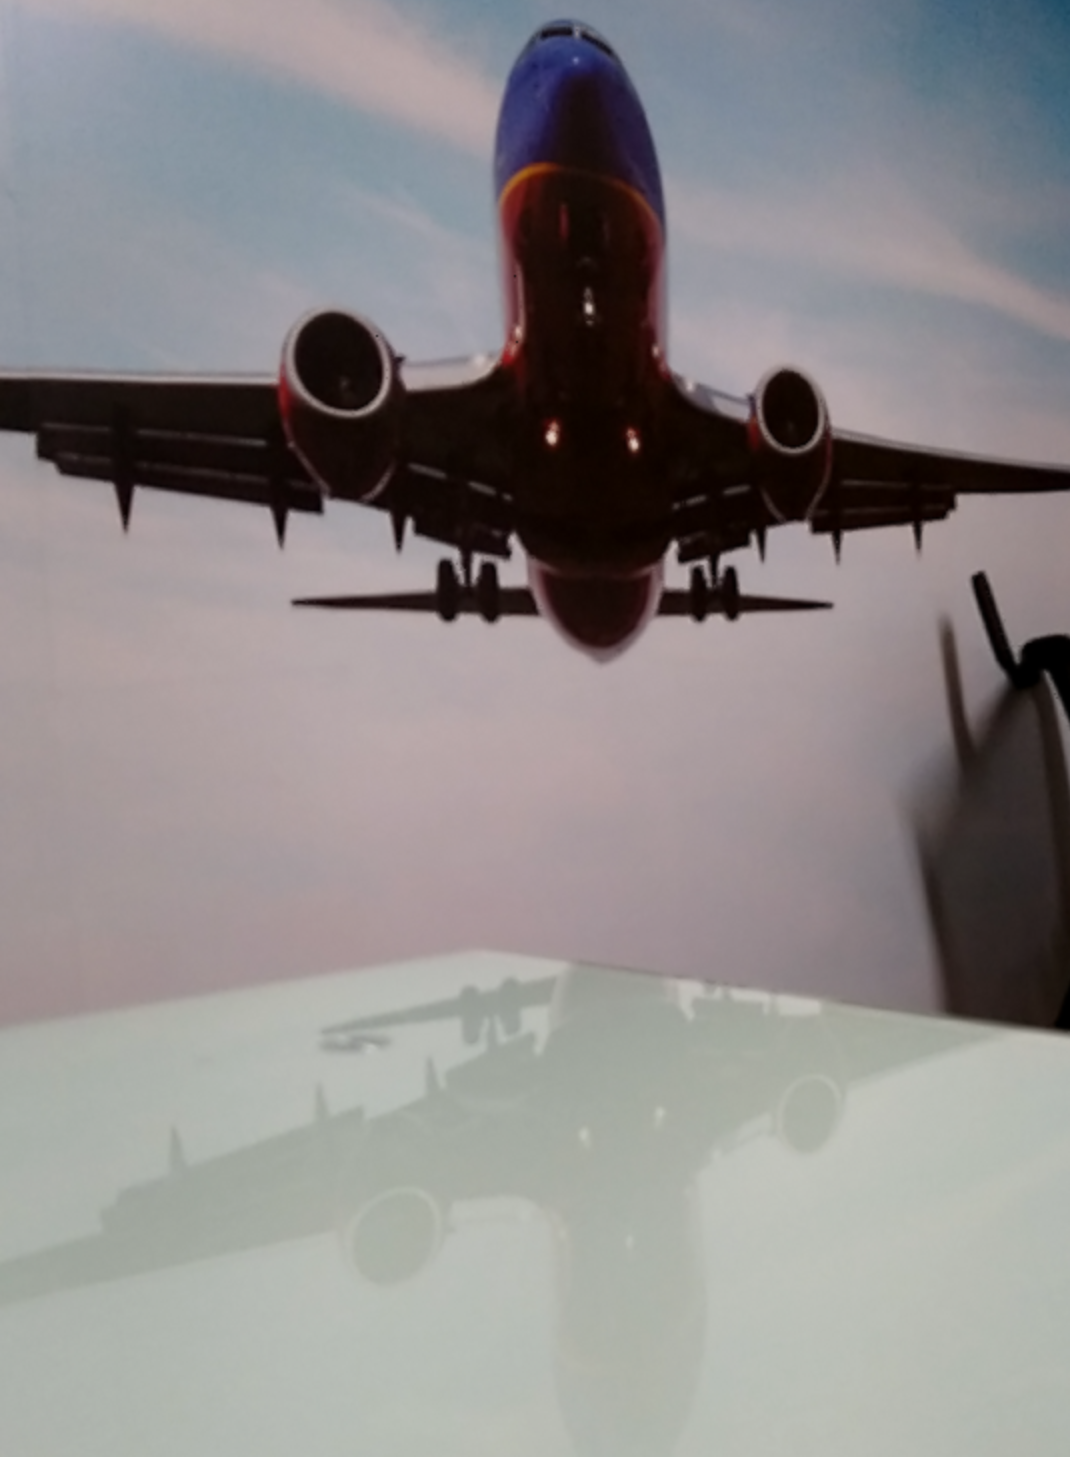
\includegraphics[width=6cm]{desarrollo/secciones/pruebas/motog6/img/VIDRIO.png}
		\caption{Malla de puntos no detectada en vidrio}
		\label{fig:motog6vidrio}
	\end{minipage}\hfill
\end{figure}

\textbf{\\Memoria de objetos} \par
Tras perder el enfoque de la cámara, al volverlo a tener, todos los objetos virtuales se volvieron a mostrar en el entorno virtual en la misma posición en la que habían sido puestos.

\textbf{Capacidad máxima de objetos} \par
Se colocaron 100 objetos virtuales en escena sin que la aplicación perdiera rendimiento. Todo funcionaba con total fluidez.

\begin{figure}[H]
	\begin{minipage}{0.48\textwidth}
		\centering
		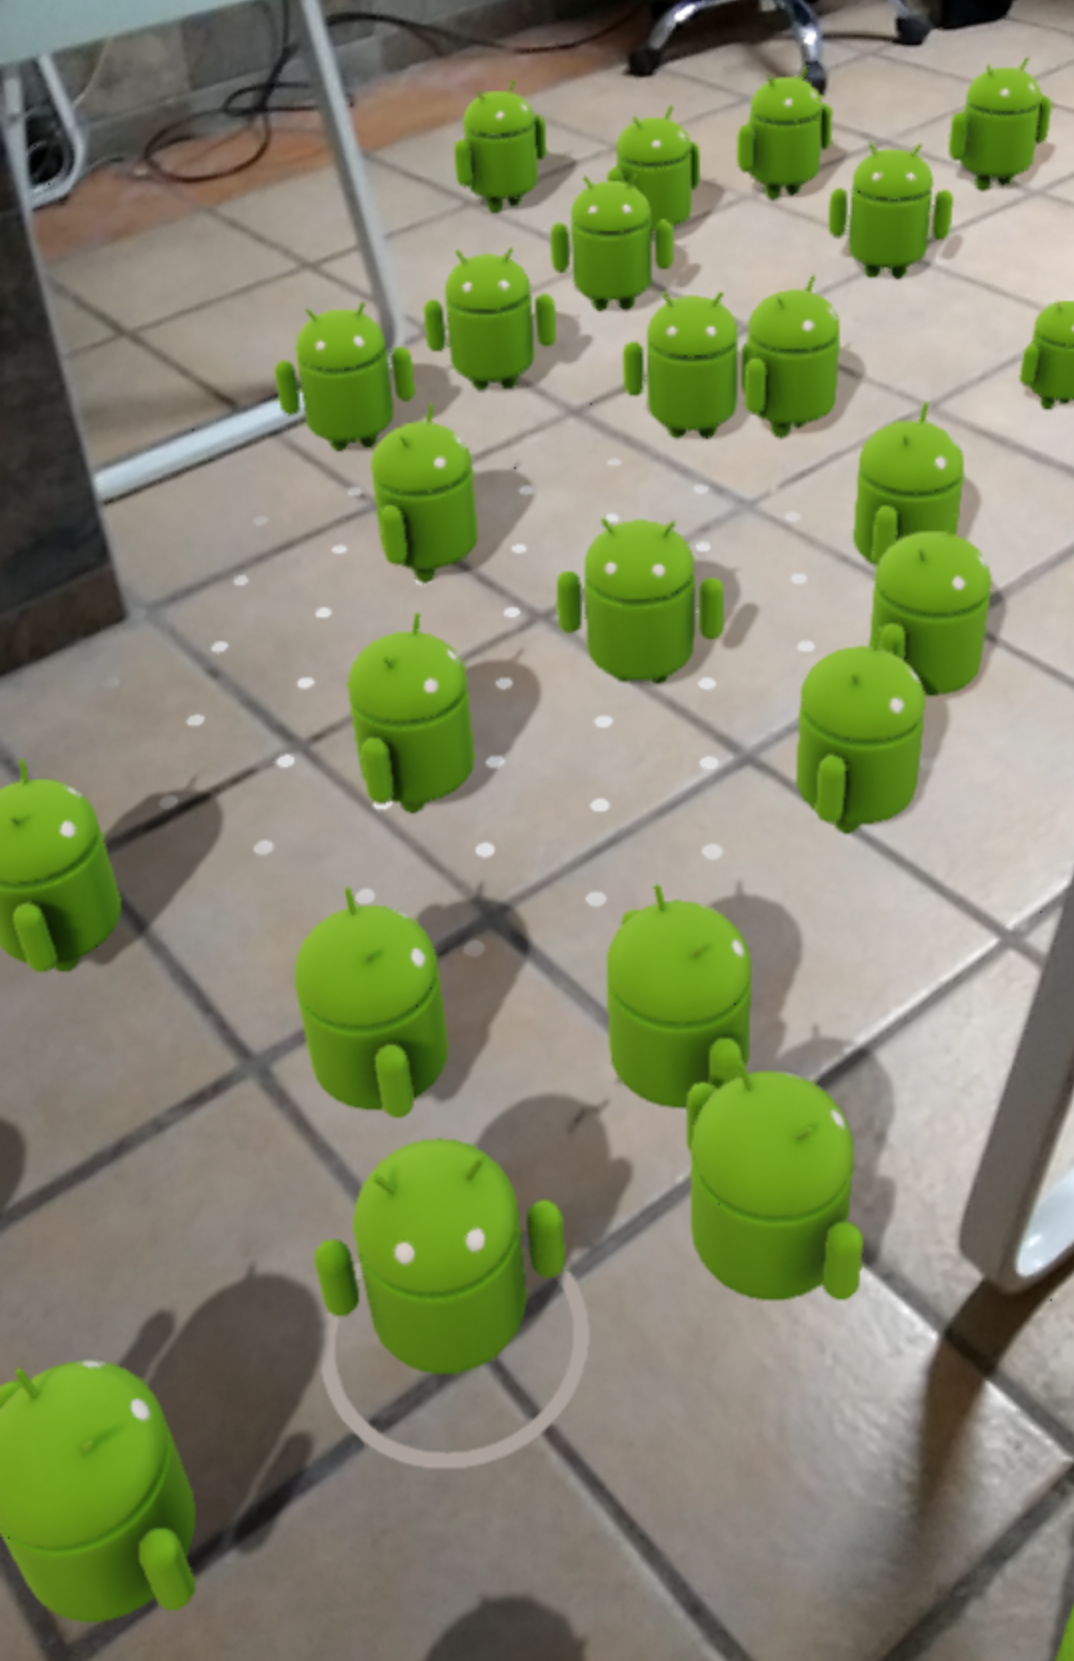
\includegraphics[width=5cm]{desarrollo/secciones/pruebas/motog6/img/CANTIDAD.png}
		\caption{Gran cantidad de objetos en escena}
		\label{fig:motog6escena}
	\end{minipage}\hfill
	\begin{minipage}{0.48\textwidth}
		
		\centering
		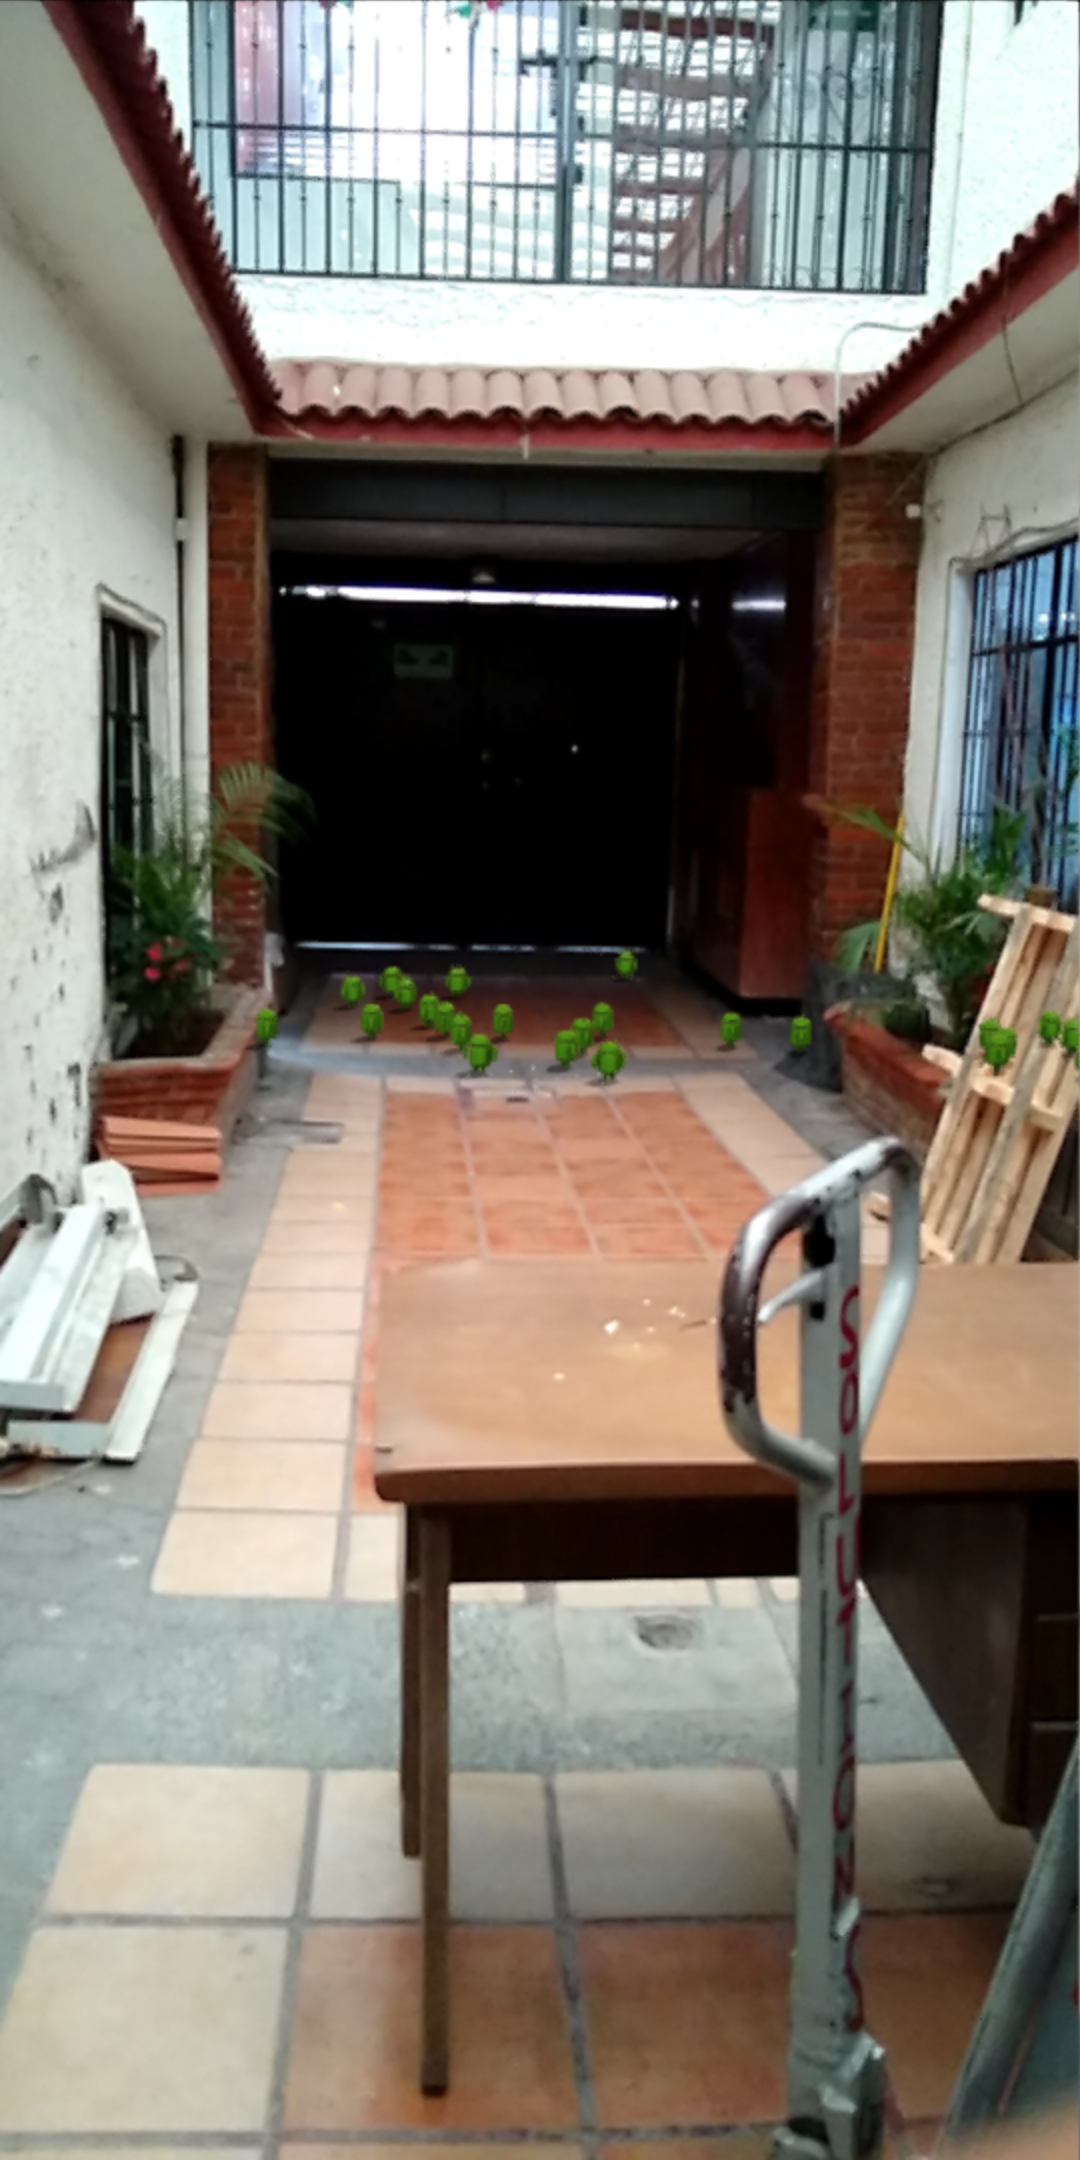
\includegraphics[width=5cm]{desarrollo/secciones/pruebas/motog6/img/DISTANCIA.png}
		\caption{Objetos puestos a gran distancia}
		\label{fig:motog6edistancia}
	\end{minipage}\hfill
\end{figure}

\textbf{Distancia} \par
Se colocó un objeto, después la cámara fue alejada hasta una distancia de \textbf{11.22m.} A esa distancia los objetos comenzaron a verse pixeleados, además comenzaron a desaparecer y reaparecer de forma intermitente.


\noindent
\subsubsection{ARcore}
\begin{table}[H]
	\centering
	\begin{tabular}{|c|c|}
		\hline
		\multicolumn{2}{|c|}{Especificaciones de prueba}   \\ \hline
		\textbf{DISPOSITIVO}              & Moto G6 XT1925 \\ \hline
		\textbf{FECHA}                    & 2018/08/25     \\ \hline
		\textbf{VERSIÓN DE SCENEFORM SDK} & V1.4.0         \\ \hline
		\textbf{VERSIÓN DE ARCORE SDK}    & V1.4.0         \\ \hline
		\textbf{VERSIÓN DE ANDROID}       & V8.0.0 (Oreo)  \\ \hline
	\end{tabular}
	\captionsetup{justification=centering}
	\caption{Especificaciones de prueba Arcore en Moto G6}
\end{table}

\textbf{Posición cardinal} \par
El objeto virtual se pudo apreciar con claridad desde los cuatro puntos cardinales y la vista superior. El ángulo de visualización del objeto al mover la cámara cambiaba a la perfección, dando una buena percepción de realismo.

%%IMAGENES DE PUNTOS CARDINALES
\begin{figure}[!htbp]
	\begin{minipage}{0.48\textwidth}
	\centering
		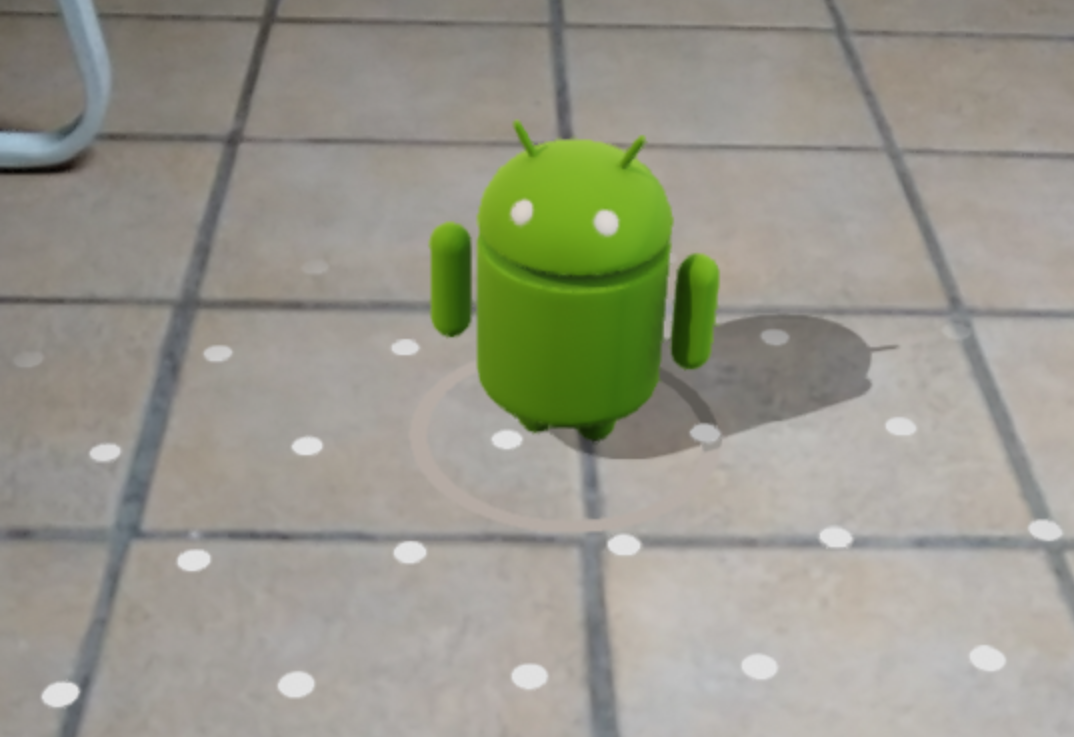
\includegraphics[width=8cm]{desarrollo/secciones/pruebas/motog6/img/NORTE.png}
		\caption{Posición Norte}
		\label{fig:motog6norte}
	\end{minipage}\hfill
	\begin{minipage}{0.48\textwidth}
	\centering
	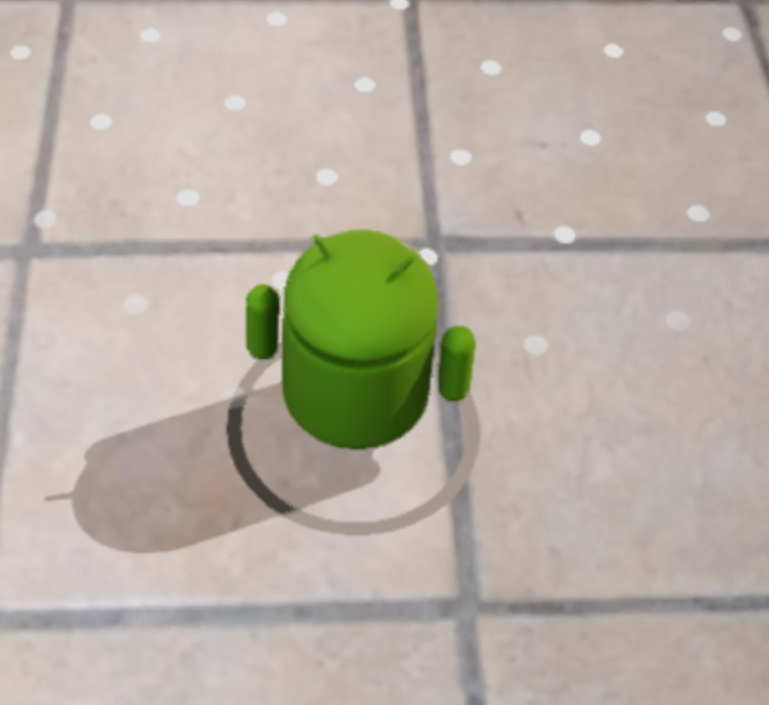
\includegraphics[width=8cm]{desarrollo/secciones/pruebas/motog6/img/SUR.png}
	\caption{Posición Sur}
	\label{fig:motog6sur}
	\end{minipage}\hfill
\end{figure}

\begin{figure}[!htbp]
	\begin{minipage}{0.48\textwidth}
		\centering
		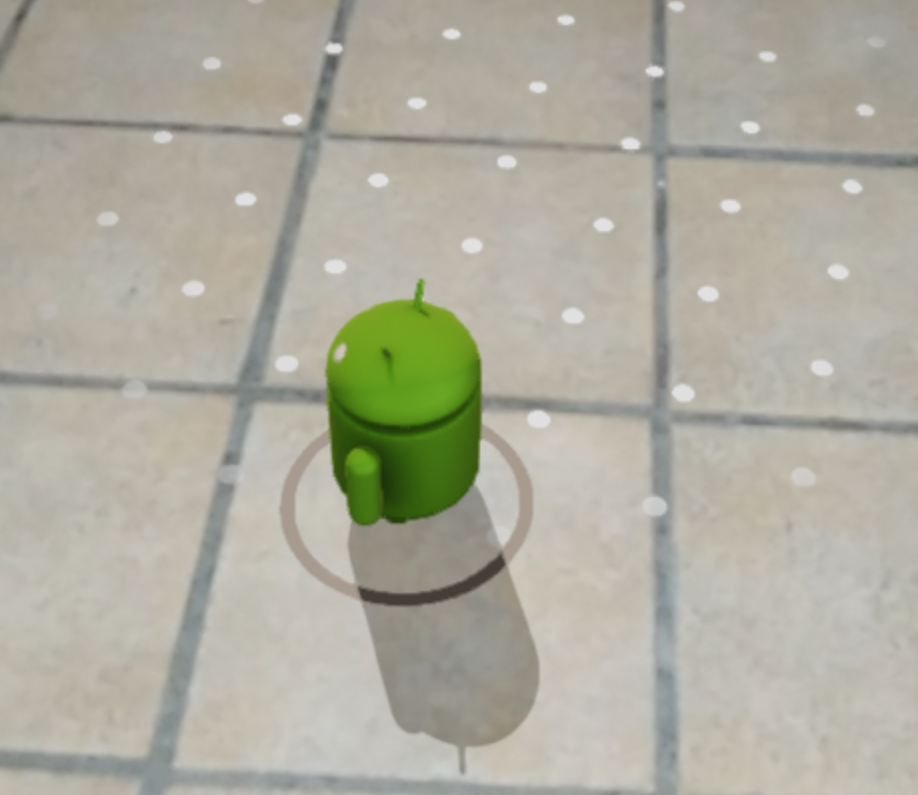
\includegraphics[width=8cm]{desarrollo/secciones/pruebas/motog6/img/ESTE.png}
		\caption{Posición Este}
		\label{fig:motog6norte}
	\end{minipage}\hfill
	\begin{minipage}{0.48\textwidth}
		\centering
		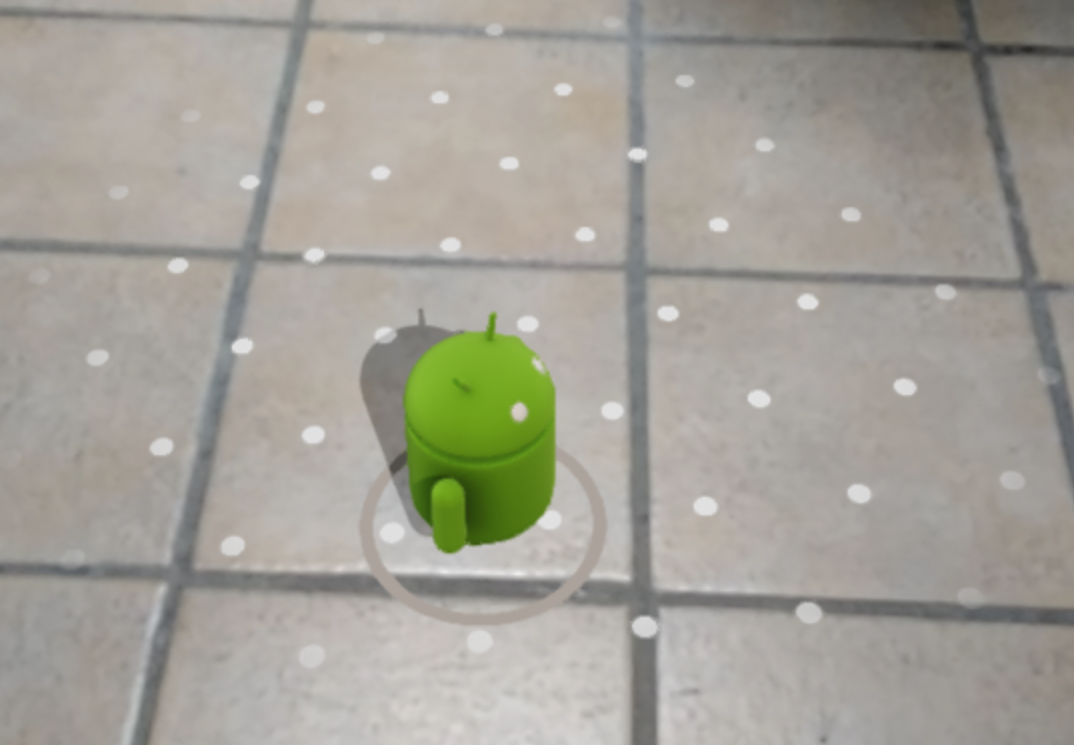
\includegraphics[width=8cm]{desarrollo/secciones/pruebas/motog6/img/OESTE.png}
		\caption{Posición Oeste}
		\label{fig:motog6oeste}
	\end{minipage}\hfill
\end{figure}

\textbf{Tamaño relativo} \par
Al acercar o alejar la cámara el objeto virtual variaba su tamaño de forma adecuada, como si el objeto realmente estuviera en la posición donde fue superpuesto.


\begin{figure}[!htbp]
	\begin{minipage}{0.48\textwidth}
		\centering
		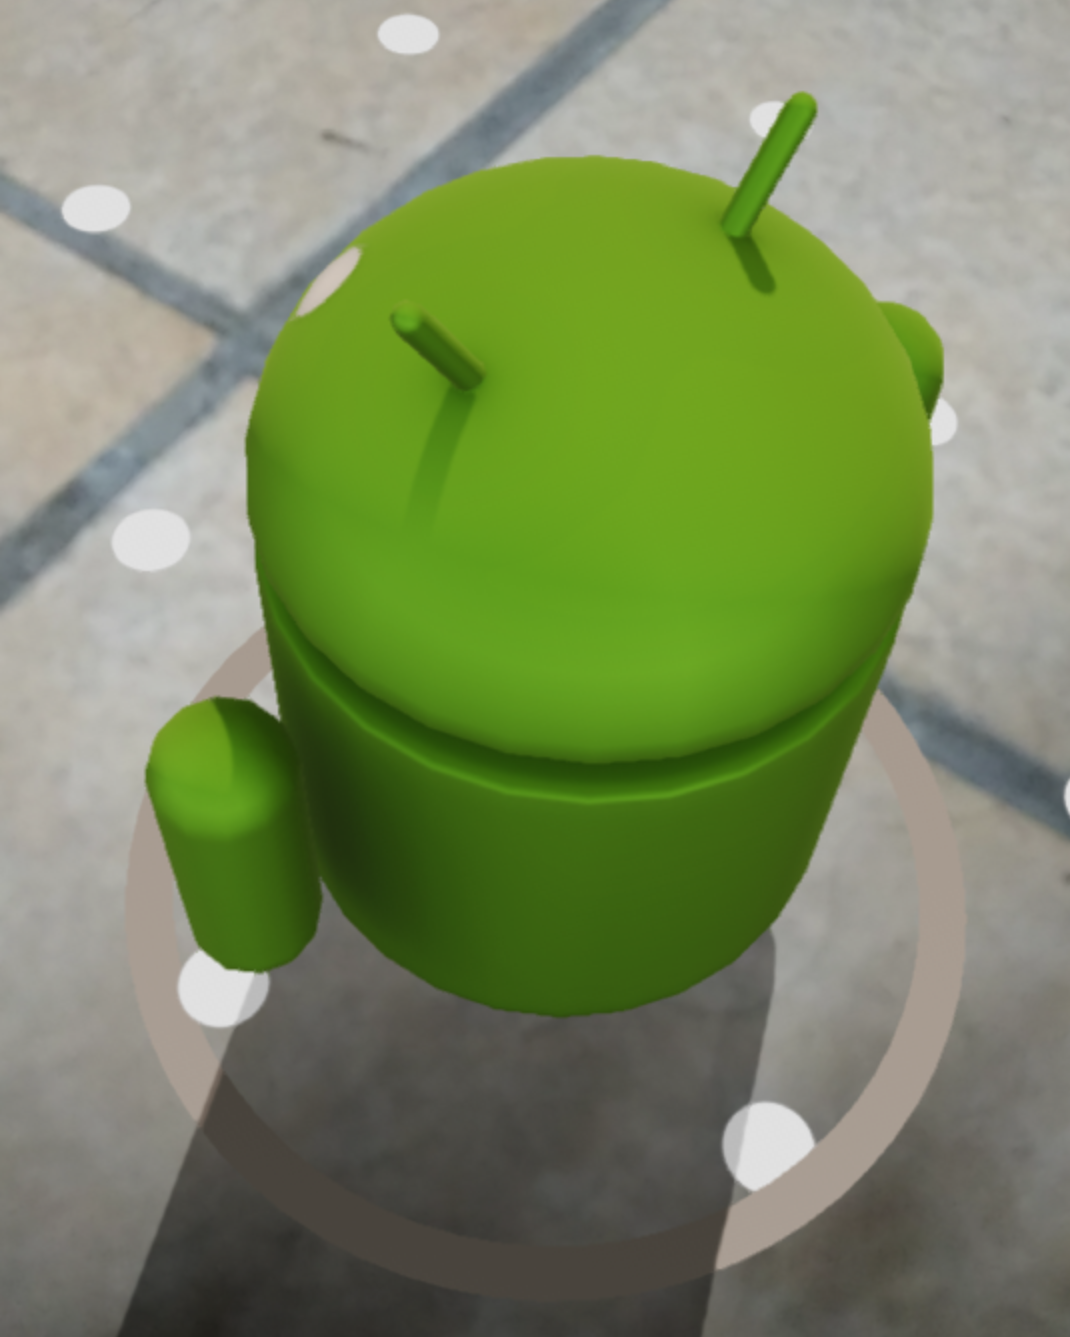
\includegraphics[width=8cm]{desarrollo/secciones/pruebas/motog6/img/CERCA.png}
		\caption{Objeto visto de cerca}
		\label{fig:motog6cerca}
	\end{minipage}\hfill
	\begin{minipage}{0.48\textwidth}
		\centering
		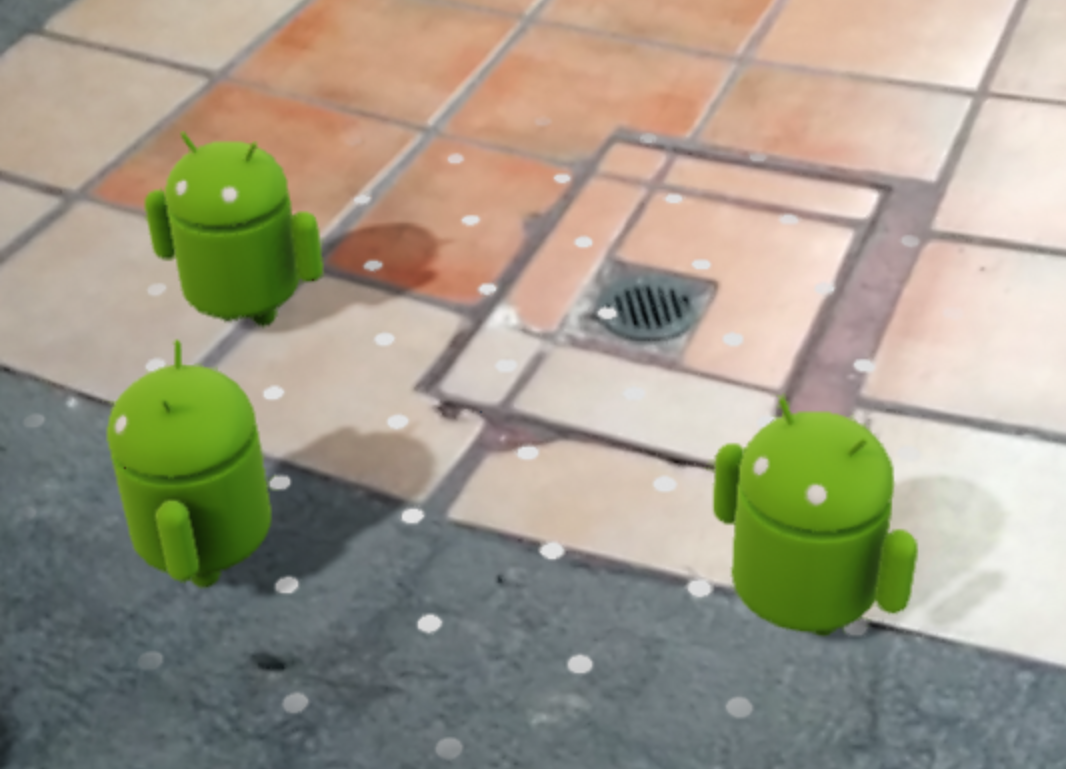
\includegraphics[width=8cm]{desarrollo/secciones/pruebas/motog6/img/LUZALTA.png}
		\caption{Luz alta}
		\label{fig:motog6lalta}
	\end{minipage}\hfill
\end{figure}

\textbf{Luminosidad} \par
Al poner el objeto virtual en entornos con diferente cantidad de luz, la cantidad de luz en el objeto virtual también variaba. En un entorno con ausencia casi total de luz el objeto apenas era perceptible, mientras que en un entorno con bastante luz, el objeto se veía altamente iluminado.

\begin{figure}[!htbp]
	\begin{minipage}{0.48\textwidth}
		\centering
		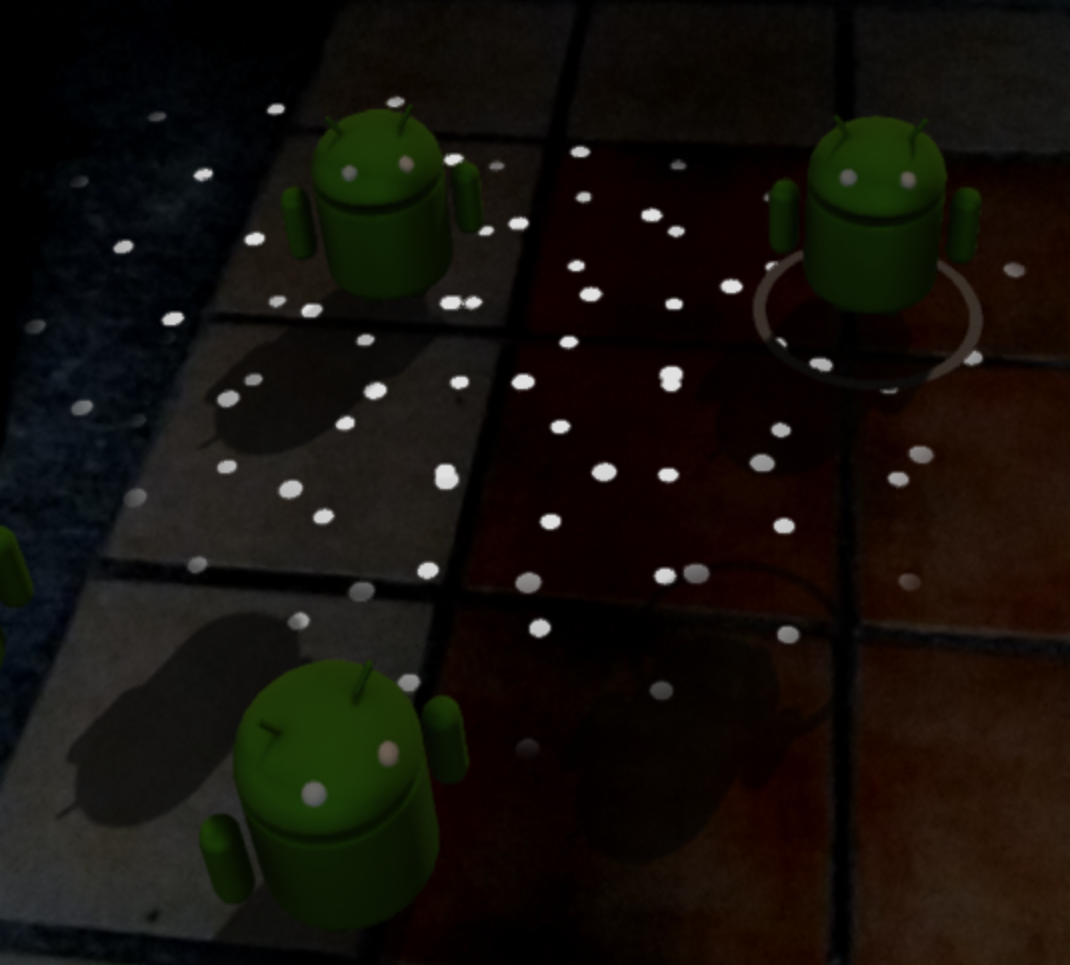
\includegraphics[width=8cm]{desarrollo/secciones/pruebas/motog6/img/LUZBAJA.png}
		\caption{Luz baja}
		\label{fig:motog6lbaja}
	\end{minipage}\hfill
	\begin{minipage}{0.48\textwidth}
		\centering
		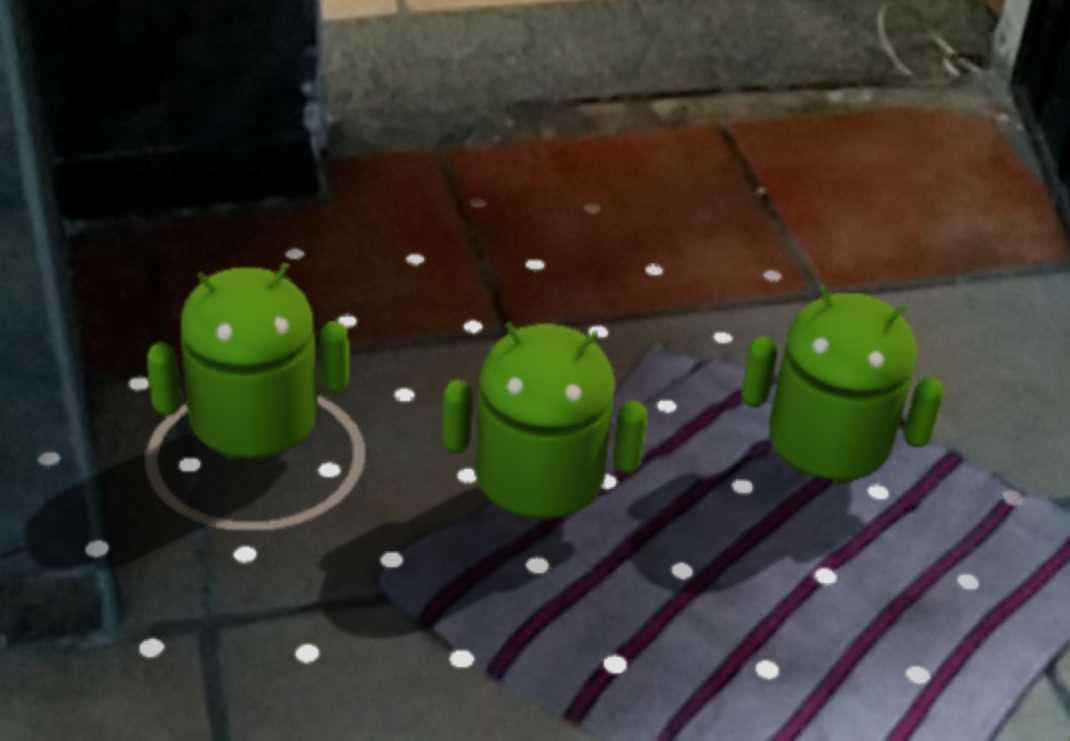
\includegraphics[width=8cm]{desarrollo/secciones/pruebas/motog6/img/LUZMEDIA.png}
		\caption{Luz media}
		\label{fig:motog6lmedia}
	\end{minipage}\hfill
\end{figure}

\textbf{Superficie} \par
Se probó posicionar el objeto virtual en cuatro superficies: concreto gris, concreto blanco, azulejo y vidrio.\par
Concreto gris.- El objeto se pudo posicionar a la perfección.\par
Concreto blanca.- El objeto no se pudo posicionar. La maya de puntos ni si quiera era detectada en ésta superficie debido a la ausencia de texturas.\par
Azulejo.- El objeto se pudo posicionar a la perfección.\par
Vidrio.- El objeto no pudo ser posicionado en ésta superficie debido a las propiedades reflejantes que posee.\par

\begin{figure}[!htbp]
	\begin{minipage}{0.48\textwidth}
		\centering
		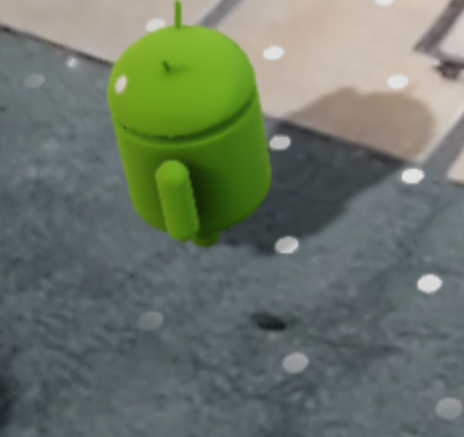
\includegraphics[width=8cm]{desarrollo/secciones/pruebas/motog6/img/CONCRETO.png}
		\caption{Objeto colocado en concreto}
		\label{fig:motog6concreto}
	\end{minipage}\hfill
	\begin{minipage}{0.48\textwidth}
		\centering
		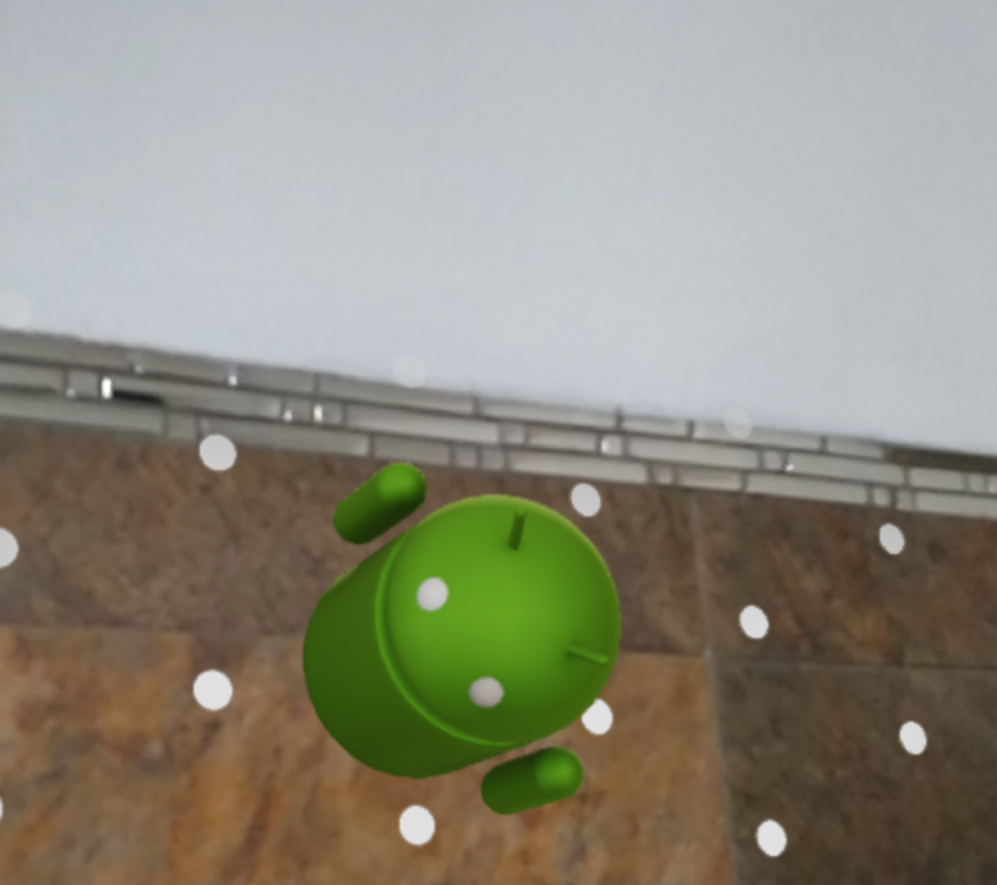
\includegraphics[width=8cm]{desarrollo/secciones/pruebas/motog6/img/SUPBLANCA.png}
		\caption{Objeto colocado en superficie blanca}
		\label{fig:motog6supblanca}
	\end{minipage}\hfill
\end{figure}

\begin{figure}[H]
	\begin{minipage}{0.48\textwidth}
		\centering
		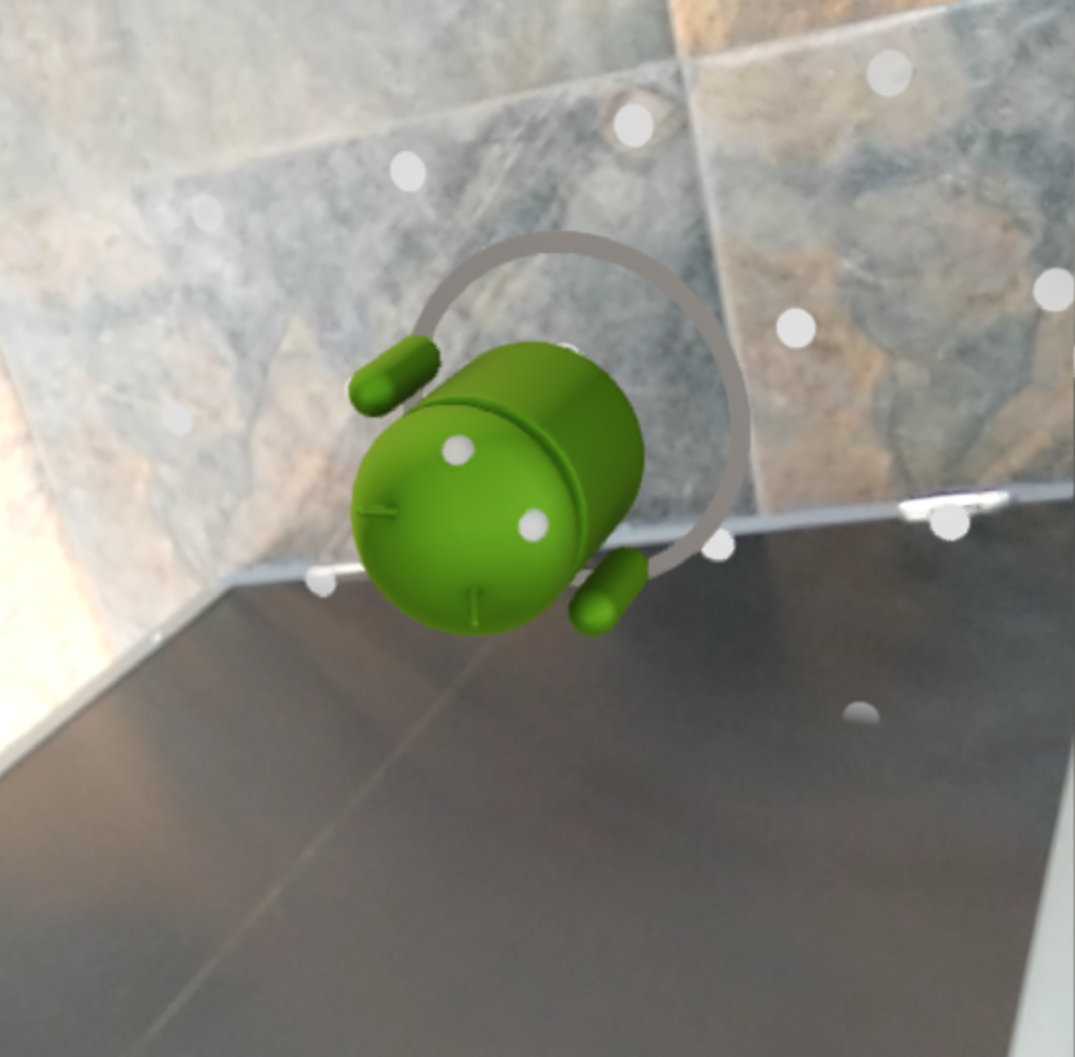
\includegraphics[width=8cm]{desarrollo/secciones/pruebas/motog6/img/SUPERFICIENEGRA.png}
		\caption{Malla de puntos no detectada en superficie negra}
		\label{fig:motog6supnegra}
	\end{minipage}\hfill
	\begin{minipage}{0.48\textwidth}
		\centering
		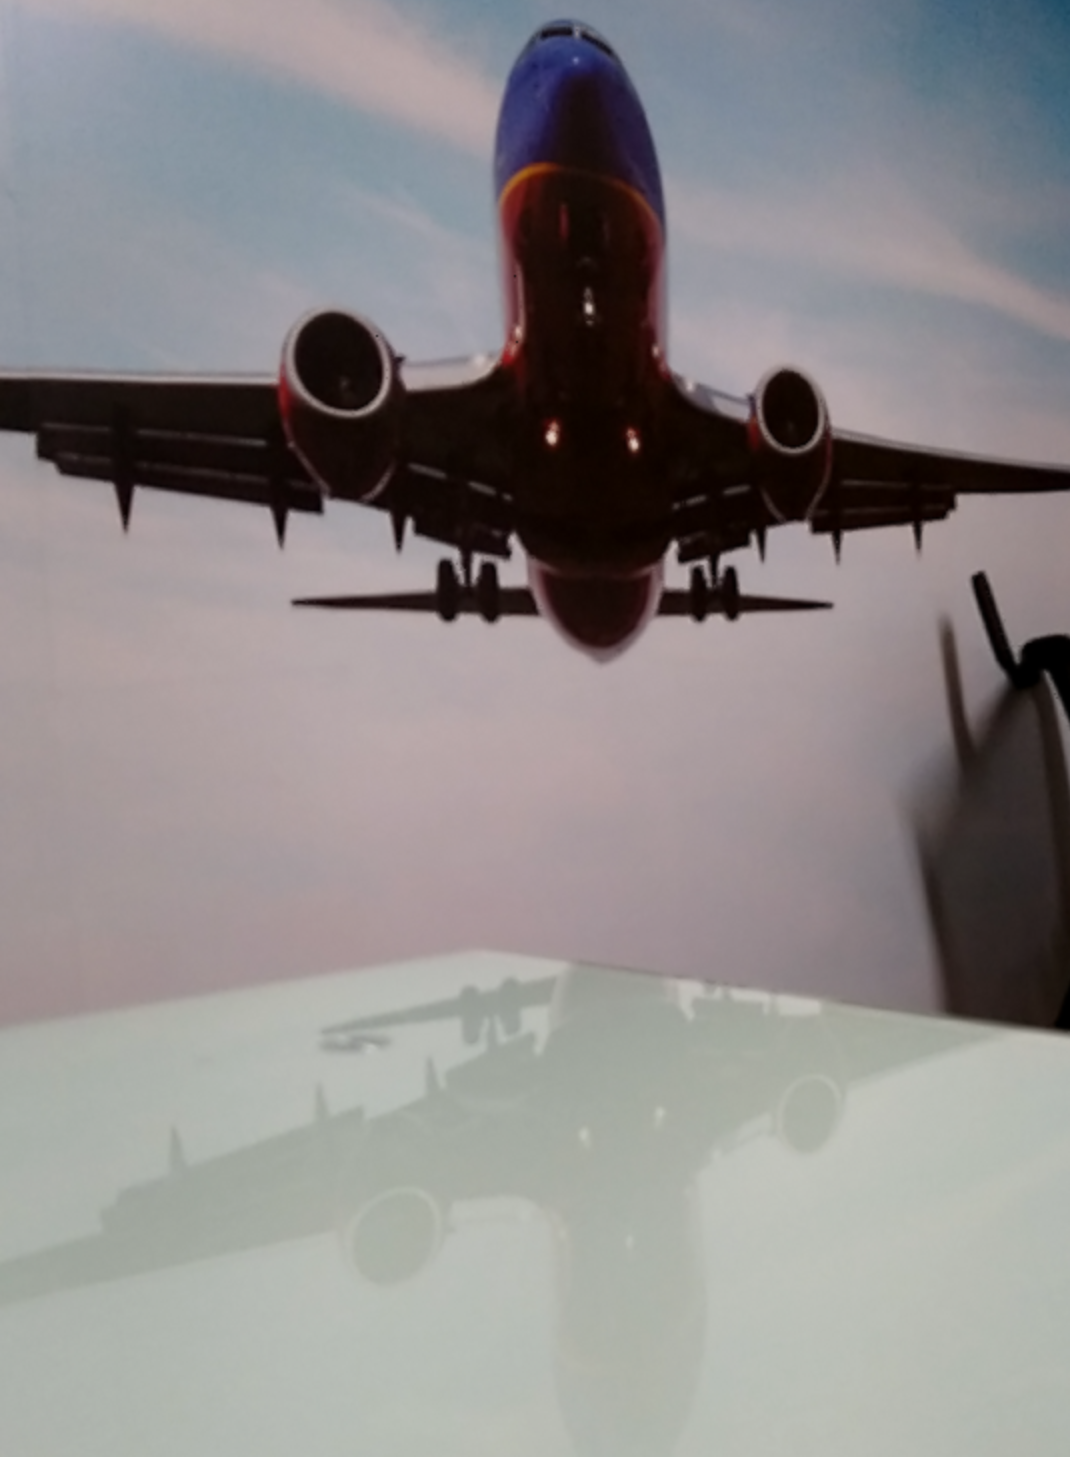
\includegraphics[width=6cm]{desarrollo/secciones/pruebas/motog6/img/VIDRIO.png}
		\caption{Malla de puntos no detectada en vidrio}
		\label{fig:motog6vidrio}
	\end{minipage}\hfill
\end{figure}

\textbf{\\Memoria de objetos} \par
Tras perder el enfoque de la cámara, al volverlo a tener, todos los objetos virtuales se volvieron a mostrar en el entorno virtual en la misma posición en la que habían sido puestos.

\textbf{Capacidad máxima de objetos} \par
Se colocaron 100 objetos virtuales en escena sin que la aplicación perdiera rendimiento. Todo funcionaba con total fluidez.

\begin{figure}[H]
	\begin{minipage}{0.48\textwidth}
		\centering
		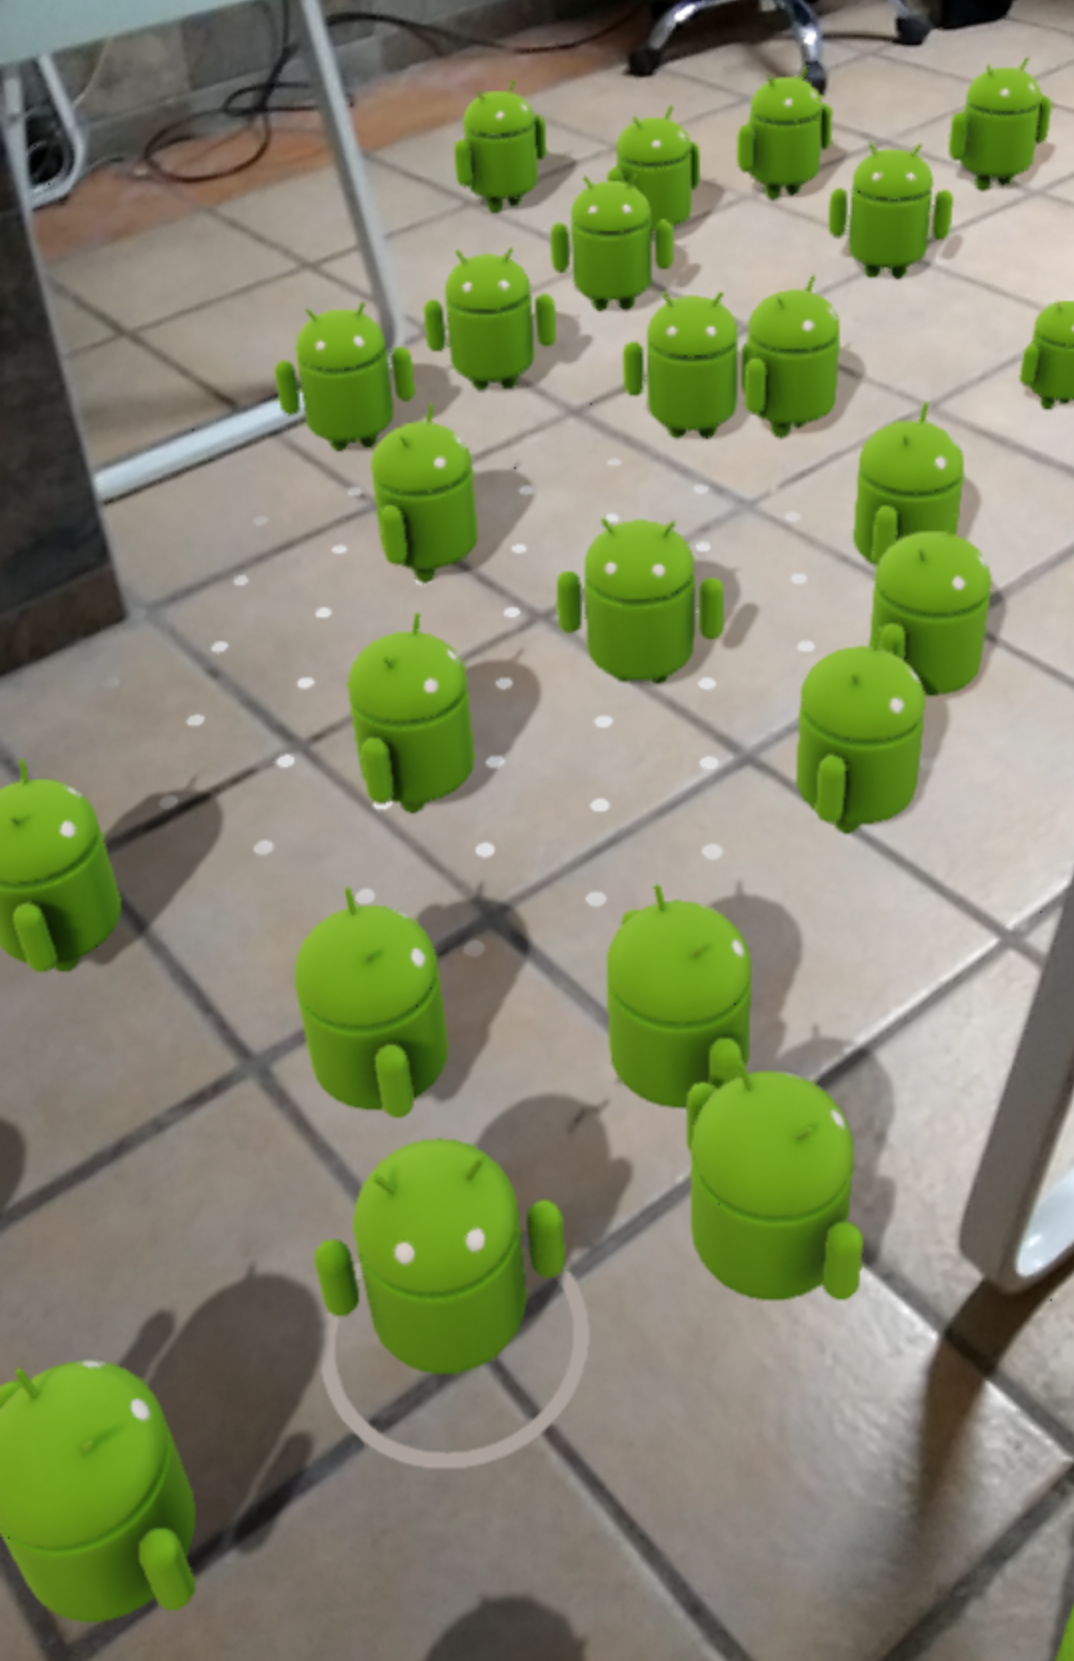
\includegraphics[width=5cm]{desarrollo/secciones/pruebas/motog6/img/CANTIDAD.png}
		\caption{Gran cantidad de objetos en escena}
		\label{fig:motog6escena}
	\end{minipage}\hfill
	\begin{minipage}{0.48\textwidth}
		
		\centering
		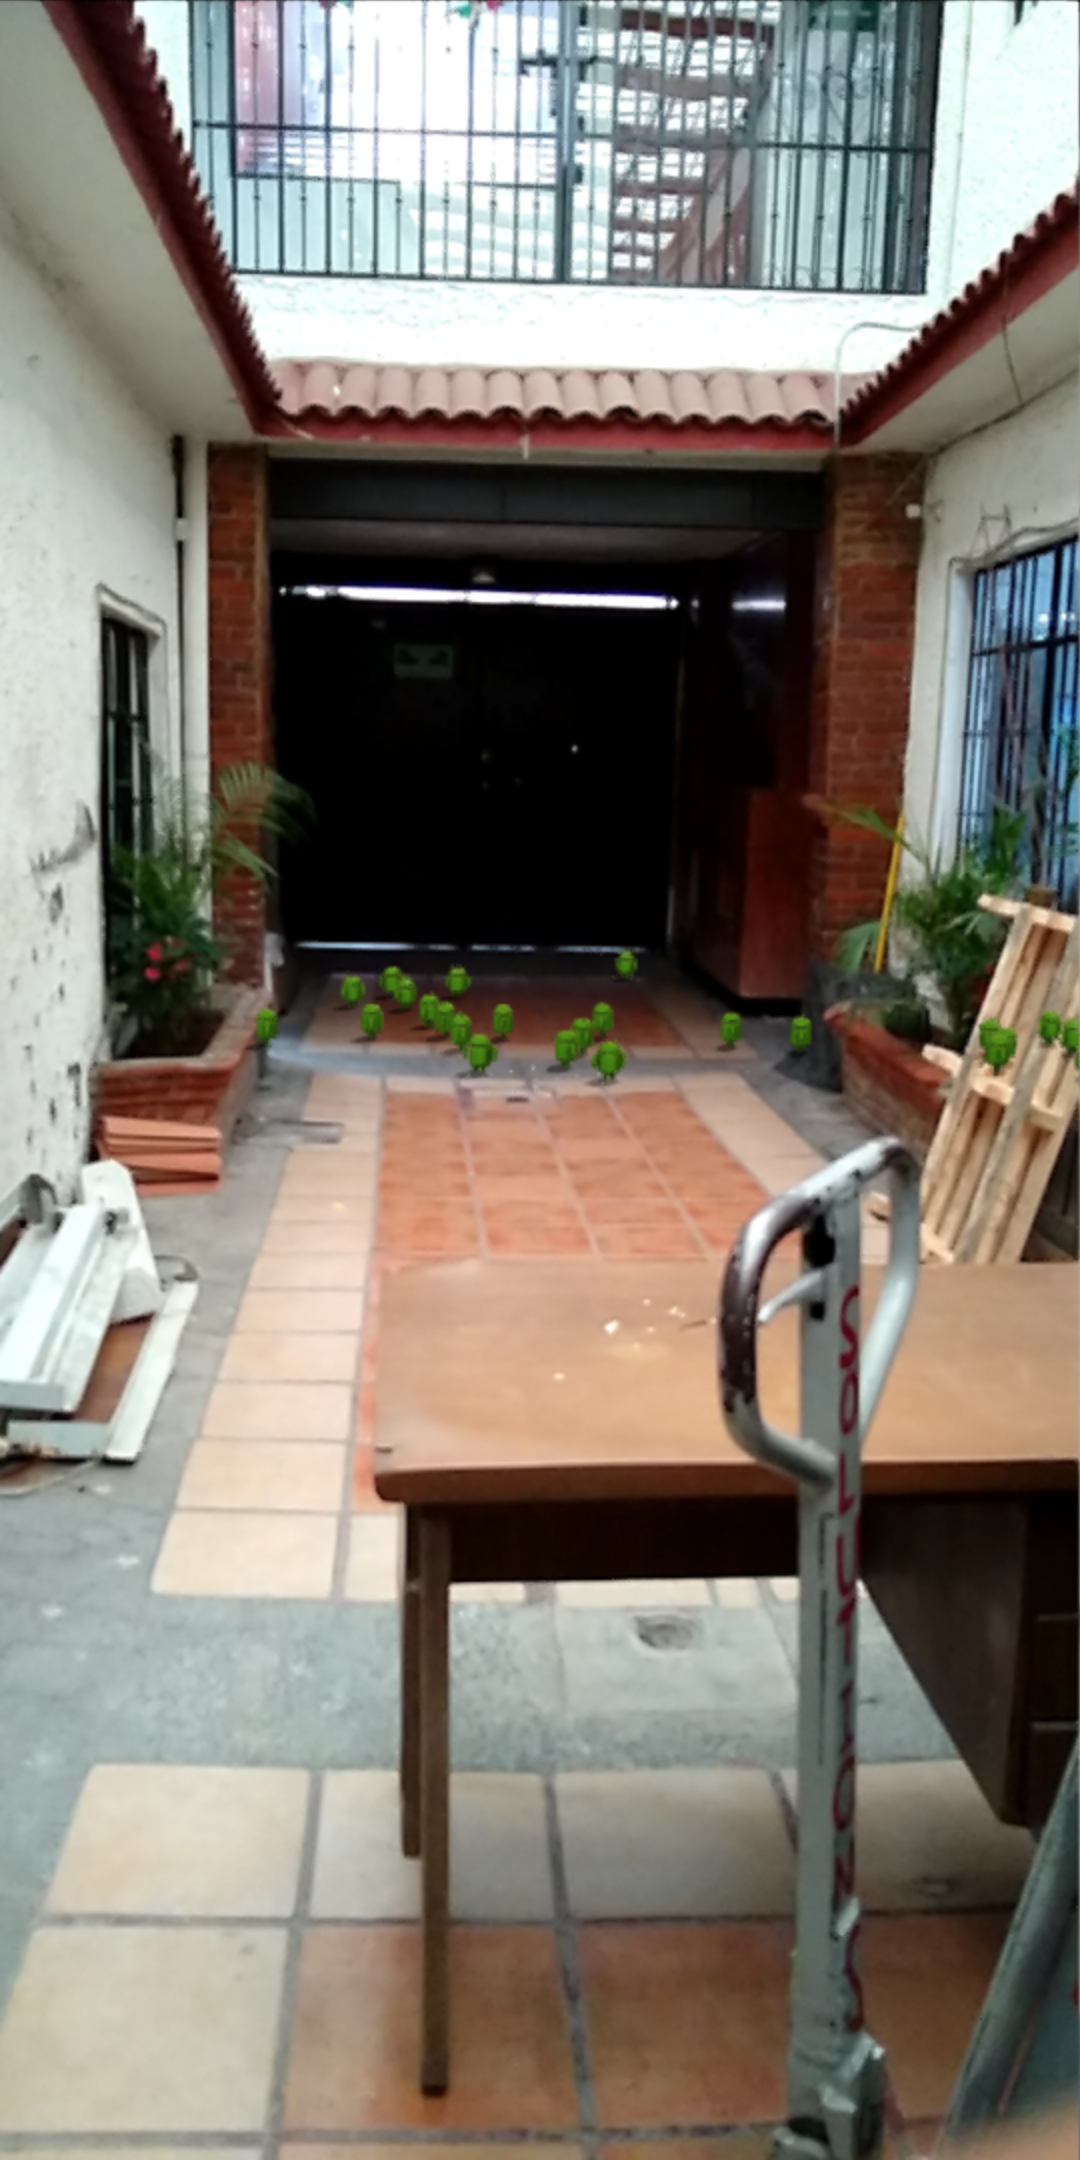
\includegraphics[width=5cm]{desarrollo/secciones/pruebas/motog6/img/DISTANCIA.png}
		\caption{Objetos puestos a gran distancia}
		\label{fig:motog6edistancia}
	\end{minipage}\hfill
\end{figure}

\textbf{Distancia} \par
Se colocó un objeto, después la cámara fue alejada hasta una distancia de \textbf{11.22m.} A esa distancia los objetos comenzaron a verse pixeleados, además comenzaron a desaparecer y reaparecer de forma intermitente.


\noindent

\subsubsection{Conclusión de pruebas de contexto}
Tras las pruebas de contexto realizadas con ARCore y Vuforia, se tomó la decisión de desarrollar el proyecto con ARCore por las siguientes razones:
\begin{itemize}
	\item Vuforia presentó intermitencia en las pruebas de posición cardinal.
	\item Vuforia depende de un marcador físico para posicionar el objeto.
	\item La dependencia de Vuforia al marcador físico elimina la capacidad de memoria de objetos.
	\item Vuforia en ambientes con luz muy baja es incapaz de funcionar.
	\item Con Vuforia se requieren imprimir tantos marcadores físicos como objetos se deseen visualizar. Es decir, si se quieren mostrar 30 muebles en escena, es necesario imprimir y posicionar los 30 marcadores en el entorno físico.
\end{itemize}
\newpage

\subsubsection{Establecimiento de interesados}
\textbf{Desarrolladores} \par
Para poder construir la aplicación requeriremos desarrolladores que puedan diseñar la arquitectura que tendrá la aplicación y programarla. Los tres desarrolladores que estarán trabajando en el proyecto son Gerardo Aramis Cabello Acosta, Martín Alejandro Carrillo Mendoza y Saúl del Pilar Morales. Su intervención se requerirá en todas las iteraciones del proyecto desde la I a la IX.\par
\textbf{Directores} \par
Los directores serán los encargados de supervisar los avances del proyecto en cada iteración. También serán elementos de apoyo a los que los desarrolladores podrán acudir en caso de tener alguna duda o complicación. Su intervención se requerirá durante todo el desarrollo del proyecto desde la iteración I a la iteración IX.\par
\textbf{Sinodales} \par
Serán quienes evaluarán el proyecto al terminar los entregables de TT I y TT II. Su intervención se requerirá al finalizar las iteraciones IV y IX.\par
\textbf{Arquitecto} \par
Se requiere contactar a un arquitecto que tenga conocimientos en antropometría con el objetivo de poder obtener una retroalimentación del proyecto. Ésta retroalimentación nos servirá para poder mejorar la aplicación modificando, añadiendo o removiendo características. Su intervención se requerirá en la fase de inicialización y en la fase de planeación de la iteración V, que será la fase inmediata después de presentar TT I.\par
\textbf{Diseñador de interiores} \par
Se requiere para obtener una retroalimentación más precisa, dado que es uno de los dos principales usuarios del sistema. Su intervención se requerirá en la fase de planeación de la iteración V, que será la inmediata después de presentar TT I; también se requerirá su intervención en todo el proceso de desarrollo posterior a la iteración V.\par

\subsubsection{Alcance}
Se desarrollará una aplicación móvil para dispositivos móviles que usen Android como sistema operativo en su versión 7.0 en adelante y que se encuentren dentro de la lista especificada por la \textit{Tabla 2.6}\par
El objetivo de la aplicación será lograr que el proceso de diseño de interiores sea más sencillo y rápido, esto a través de la eliminación y reducción de etapas del proceso implicado (véase \textit{Figura 1.1}).
La aplicación cumplirá las siguientes funciones:\par
\begin{itemize}
	\item Tendrá un login, el cual tras la autenticación, permitirá guardar los escenarios que se vayan generando con sus respectivas fotografías.
	\item Tendrá una opción alternativa para iniciar la aplicación sin pasar por un proceso de autenticación. En este caso sólo se podrá generar un entorno virtual con AR pero no se podrá guardar el escenario.
	\item Tendrá un catálogo de muebles modelados y renderizados en 3D
	\item La aplicación podrá incluir hasta 100 muebles en escena al mismo tiempo.
	\item Será posible cambiar las texturas de los muebles puestos en escena.
	\item Los objetos puestos en escena tendrán posición relativa.
	\item Los objetos puestos en escena tendrán una variación dinámica de luz, esto es, que conforme cambie la luz en el ambiente real, también lo hará de forma virtual en los objetos superpuestos.
	\item La superposición de objetos no requerirá el uso hardware externo o marcadores físicos.
	\item Será posible mover los muebles de lugar aún después de ser puestos en escena.
	\item La aplicación podrá tomar fotografías de los escenarios de realidad aumentada que vaya generando el usuario.
	\item La aplicación permitirá asociar las fotografías tomadas a escenarios específicos. \textit{v.g. ``Diseño de interiores - Casa Loma Bonita"}
	\item La aplicación permitirá crear proyectos el cual se conformará por varios escenarios, para el caso en el que un diseñador realice varios diseños de interiores para un mismo cliente.
\end{itemize}
\noindent
El desarrollo del proyecto será finalizado en mayo de 2019.
\subsubsection{Establecimiento de proyecto}
El proyecto será realizado en nueve iteraciones hasta el entregable de TT II. Dado que la metodología es ágil basada en Extreme Programming, dividiremos el desarrollo en dos partes, para los entregables de TT I y TT II. La primer parte comprende desde iteración uno hasta la cuatro, al final de la cual terminaremos el entregable de TT I y realizaremos nuestra presentación. A continuación se encuentran descritas cada una de la iteraciones que involucrarán el desarrollo de TT I.\par

\textbf{Iteración I} \par
En este punto ya está realizada la primer implementación de AR con la cual se realizaron las pruebas de contexto descritas anteriormente. Por lo tanto, para ésta iteración vamos a implementar un modelo 3D propio. Usaremos Blender para el modelado y renderizado de éste elemento. Al final de ésta iteración tendremos una aplicación en Android que pueda desplegar a través de AR un modelo 3D diseñado por nosotros.

\textbf{Iteración II} \par
En esta iteración vamos hacer el diseño detallado de un mueble. De igual manera el modelado y renderizado será en Blender. Al final de ésta iteración tendremos una aplicación en Android que pueda desplegar a través de AR un mueble. El entregable de ésta iteración es el equivalente al planeado en el protocolo para TT I.

\textbf{Iteración III} \par
En esta iteración vamos a desarrollar el backend de la aplicación para poder realizar el login, registro de cuenta, recuperación de contraseña y el guardado de los escenarios que se vayan generando en la realidad aumentada. Al final de ésta iteración se tendrá el backend totalmente funcional para conectarlo con la aplicación a través del protocolo HTTP.

\textbf{Iteración IV} \par
En esta iteración vamos a generar varios modelos de muebles y presentarlos en la aplicación de tal forma que puedan ser seleccionables y puedan ser posicionados de forma individual en el mismo escenario. También vamos a implementar la funcionalidad de tomar una foto del entorno virtual generado y almacenarla en el dispositivo.

\textbf{Iteración V} \par
En esta iteración vamos a generar el acceso a usuarios a la aplicación, lo cual implica desarrollar un login, el registro de cuentas y un método de recuepración de contraseña.

\textbf{Iteración VI} \par
En esta iteración vamos a desarrollar la forma de gestionar proyectos de clientes, desde los cuales se podrán crear escenarios.

\textbf{Iteración VII} \par
En esta iteración desarrollaremos las funciones necesarias para que un usuario puede generar un escenario, así como actualizar su información general, borrarlo, y visualizar los escenarios que haya generado (por proyecto).

\textbf{Iteración VIII} \par
En esta iteración se desarrollará una plataforma web desde la cual los usuarios podrán subir muebles a su cuenta, los cuales podrá utilizar dentro de la aplicación. Asimismo podrá gestionar categorías y subcategorías para tener sus muebles organizados.

\textbf{Iteración IX} \par
En ésta iteración vamos a generar varios modelos de muebles y presentarlos en la aplicación de tal forma que puedan ser seleccionables y puedan ser posicionados de forma individual en el mismo escenario. También vamos a implementar la funcionalidad de tomar una foto del entorno virtual generado y almacenarla en el dispositivo.




